% part4.tex

\part{\LaTeX{}浮动图形环境}

\section{浮动图形环境}\label{sec:floatfigure}
在使用字处理软件排版时,用户放在哪里图形就会出现在哪里\footnote{
	尽管许多字处理软件确实可以允许图形在文本周围移动(或者文本在图形周围移动),
	但是出于糟糕的软件设计以及/或者文档作者的忽略,绝大部分用户并不使用该功能。}。
但是,因为这些图形不能被分割开来,所以经常会导致糟糕的分页,将大片的空白留在页面下方。
为得到专家级的排版效果,作者不得不手工调整图形的位置。
这种工作是非常乏味的,尤其是几乎每次修改文档都得这样做一次。

为此,\LaTeX{}~提供了一个浮动图形机制来自动将图形放置到看起来合适的位置,
既能得到专家级的排版效果,又不必手工做调整图形位置的乏味的工作。
不过,它也会给那些习惯于手工调整图形的新手带来不适。
想要有效的利用浮动图形机制需要注意以下几点:
\begin{description}
	\item[不要使用依赖于图形放置位置的文本]
	
	使用如“\emph{这幅图...}”或“\emph{下面的图形...}”等短语要求所指的图形需在固定位置。
	而像~``\emph{图~5...}''~这样的短语则允许图形出现在任意位置。
	\item [放松]
	
	一些用户在发现图形没有十分准确的出现在他们所想要的位置时,往往非常着急。
	这没有必要,图形的放置是 \LaTeX{} 的工作,最好放松一些。
\end{description}

在接下来的几页中我们将介绍 \LaTeX{} 是以怎样的专业级的排版规则来决定浮动图形的位置的。
\marginpar{经验总结}
为方便起见,下面列出关于浮动图形放置的一些最常见问题的解决方法。
\begin{enumerate}
	\item 不要束缚 \LaTeX{} 的手脚。
	给出的浮动选项越多,\LaTeX{} 做的就越好。
	特别地,使用选项 \opt{[htbp]} 和 \opt{[tbp]}	就很好。
	见第~\ref{ssec:figplacement}~节。
	
	\item 很多人发现缺省的浮动参数过于严格了。下面的命令
\begin{lstlisting}
\setcounter{topnumber}{4}
\setcounter{bottomnumber}{4}
\setcounter{totalnumber}{10}
\renewcommand{\textfraction}{0.15}
\renewcommand{\topfraction}{0.85}
\renewcommand{\bottomfraction}{0.70}
\renewcommand{\floatpagefraction}{0.66}
\end{lstlisting}
	将浮动参数重新设置为更宽松的值。详见第~\ref{sec:typerule}~节。
	
	\item \LaTeX{} 允许图形浮动到当前页的顶部,
	这样会使图形在引述它的文本前出现。
	不喜欢这样做的用户可以使用~\pkgi{flafter}宏包。
	无需使用特殊的命令,只要简单地调入该宏包 \cmdonearg{usepackage}{flafter} 即可。
	
	\item 要确保图形的浮动不超过某一特定点,可调入 \pkgi{placeins} 宏包,
	并且使用 \cmdi{FloatBarrier} 命令。见第~\ref{ssec:unprocessfig}~节。
	
	\textbf{警告}:过多使用 \cmd{FloatBarrier}	命令会导致浮动位置难以控制或浮动参数不正确。
	这两种情况都是应当尽量避免的。
\end{enumerate}


\subsection{创建浮动图形}

可以通过把命令置于一个~\ei{figure}~环境中来生成浮动图形。在图形环境
中的所有内容都会被保持在一起,浮动到合式的位置以保证得到最好的分页
结果。通过使用~\ci{caption}~命令来为浮动图形自动地编号并加上标题。
例如,下面的命令将~EPS~图形~\texttt{graph.eps}~放到一个浮动图形中。
\begin{Verbatim}[xleftmargin=1cm]
\begin{figure} 
\centering 
\includegraphics[totalheight=2in]{graph.eps} 
\caption{This is an inserted EPS graphic} \label{fig:graph} 
\end{figure}

The graph in Figure~\ref{fig:graph} on Page~\pageref{fig:graph}...
\end{Verbatim}

对于图形环境,应当注意:
\begin{itemize}
	\item \ci{label}~命令和~\ci{ref}, \ci{pageref}~命令配合使用,
	可对图形标题进行交叉引用。而~\cmd{label}~命令必须紧接着~\cmd{caption}~
	命令给出。
	\item 如果一图形环境中没有使用~\cmd{caption}~命令,那么它将是一
	个没有编号的浮动图形。
	\item 如果一图形环境中使用了多个~\cmd{caption}~命令,那么它将生成
	多个一起浮动的图形。这在排版并列放置的图形(见
	第~\ref{chap:sidebyside}~章)或像第~\pageref{fig:normalcap}~页
	上图~\ref{fig:normalcap}--\ref{fig:hangcap}~那样复杂排列的
	图形时是非常有用的。
	\item 可用命令~\ci{listoffigures}~来得到一个图形目录。
	\item 缺省地,图形标题将在图形目录中列出。~\cmd{caption}~命令有一可选项
	可用来将与标题文本不同的内容加到图形目录中。如:
	\begin{Verbatim}[xleftmargin=1cm]
	\caption[List Text]{Caption Text}
	\end{Verbatim}
	会在标题中使用~\texttt{Caption Text}~而在图形目录中使用
	~\texttt{List Text}。这在使用了特别长的标题时会很有用。
	\item 图形环境(\texttt{figure})不能在段落中使用。因此也不能在
	像~\texttt{parbox}~或~\texttt{minipage}~等盒子中使用。
	\item 若一图形环境(\texttt{figure})被置于一正文段落中,
	\begin{Verbatim}[xleftmargin=1cm]
	....text text text text text text 
	\begin{figure} 
	.... 
	\end{figure} 
	text text text text text text...      
	\end{Verbatim}
	那么它在正文段落结束之前不会被处理。
\end{itemize}

\subsection{图形的放置}\label{ssec:figplacement}

图形(\texttt{figure})环境有一个可选参数项允许用户来指示图形有可能
被放置的位置。这一可选参数项可以是下列字母的任意组合。
\begin{description}
	\item [\texttt{h}] {\CJKfamily{hei} 当前位置。} 将图形放置在
	正文文本中给出该图形环境的地方。如果本页所剩的页面不够,
	这一参数将不起作用。
	\item [\texttt{t}] {\CJKfamily{hei} 顶部。} 将图形放置在页面的顶部。
	\item [\texttt{b}] {\CJKfamily{hei} 底部。} 将图形放置在页面的底部
	\realfootnote{当一幅图形被放置在页面的底部时,如果此页有脚注
		的话,它将位于所有脚注的下方。现在还没有办法来避免这种情况。}。
	\item [\texttt{p}] {\CJKfamily{hei} 浮动页。} 将图形放置在一只允许
	有浮动对象的页面上。
\end{description}

\noindent{\CJKfamily{hei} 注:}
\begin{itemize}
	\item 如果在图形环境中没有给出上述任一参数,则缺省为~\texttt{[tbp]}。
	\item 给出参数的顺序不会影响到最后的结果。因为在考虑这些参数时~\LaTeX{}~
	总是尝试以~\texttt{h-t-b-p}~的顺序来确定图形的位置。所以
	~\texttt{[hb]}~和~\texttt{[bh]}~都使~\LaTeX{}~以~\texttt{h-b}~
	的顺序来排版。
	\item 给出的参数越多,~\LaTeX{}~的排版结果就会越好。~\texttt{
		[htbp], [tbp], [htp], [tp]}~这些组合得到的效果不错。
	\item 只给出单个的参数项极易引发问题\realfootnote{实际上,~\texttt{[h]}~
		选项不可能单独使用。由于使用单个的~\texttt{[h]}~选项所导致的
		糟糕结果使得较新版本的~\LaTeX{}~自动将其改为~\texttt{[ht]}。}。
	如果该图形不适合所指定的位置,它就会被搁置并阻碍对后面的图形
	的处理。一旦这些阻塞的图形数目超过了~18~幅这一~\LaTeX{}~所能容许
	的最大值,就会产生~``Too Many Unprocessed Floats''~的错误(见
	第~\ref{sec:unprocessfig}~节)。
\end{itemize}

当~\LaTeX{}~``{\CJKfamily{kai} 试图}''~放置一浮动图形时,
\marginpar{\CJKfamily{kai}\bfseries 参见文献 \\ \cite[第~198~页]{Leslie}}
它将遵循以下规则:
\begin{enumerate}
	\item 图形只能置于由位置参数所确定的地点。
	\item 图形的放置不能造成超过版心的错误(\texttt{overfull page})。
	\item 图形只能置于当前页或后面的页中\realfootnote{因为图形可浮动到当前页
		的顶部,所以它可能会出现在它所在文本的前面。要防止出现这种情况,
		可使用~\textsf{flafter}~宏包。}。所以图形只能~``向后浮动''~而
	不能~``向前浮动''。
	\item 图形必须按顺序出现。这样只有当前面的图形都被放置好之后才能被放置。
	\begin{itemize}
		\item 只要前面有未被处理的图形,一幅图形就不会被放在当前位置。
		\item 一幅~``不可能放置''~的图形将阻碍它后面的图形的放置。直到
		文件结束或达到~\LaTeX{}~的浮动限制。参见第~\ref{sec:toomanyfig}~节。
	\end{itemize}
	同样地,一表格也只能在其前面的表格都被处理完后才能被放置。
	不过,表格在排版时是跳过图形而单独处理的。
	\item 必须符合在第~\ref{chap:typerule}~章中给出的审美条件。例如,一页上的
	浮动对象的数目不能超过~\texttt{totalnumber}。\index{totalnumber@\texttt}
	在浮动位置选项前加上一个惊叹号(如~\cmd{begin\{figure\}[!ht]})
	会使~\LaTeX{}~忽略应用于文本页的审美条件,试图用最严格的标准来
	放置浮动图形。不过,~\texttt{!}~不会影响应用于浮动页的审美条件。
\end{enumerate}

\subsection{清除未处理的浮动图形}\label{ssec:unprocessfig}

使用浮动图形的一大优势就是~\LaTeX{}~不需要在将它们放置在输入它们的
地方。~\LaTeX{}~会将它们暂时保存,在更合适的地点加以放置。当一浮动
图形已被~\LaTeX{}~读入,但还没有将它放到页面上时,这一图形被称为
~``未处理浮动图形''。虽然~\LaTeX{}~通常对浮动图形的处理很好,但有时
还是需要强迫~\LaTeX{}~去处理那些未处理的浮动图形。

下面的三个方法都可以用来清除未处理的浮动图形。这些命令必须分开使用。
同时,过多地使用这些命令会使得你有时得自己来管理浮动图形的位置或
意味着浮动图形的放置参数是错误的(见第~\ref{chap:typerule}~章)。

\begin{description}
	\item [clearpage] \mbox{} \\
	最基本的用来清除未处理的浮动图形的方法就是使用~\ci{clearpage}~
	命令。它可让~\LaTeX{}~排版所有未处理的浮动图形并开始一新页。
	尽管这一命令很有效,但它也常常导致页面的下方出现很大的空白。
	\item [FloatBarrier] \mbox{} \\
	对于大多数情况,最好的方法是使用~\textsf{placeins}~宏包提供
	的~\cmd{FloatBarrier}~命令。使用~\textsf{placeins}~宏包的方法
	如下:
	\begin{itemize}
		\item \cmd{FloatBarrier}~使所有未处理的浮动图形立即被处理。
		与~\cmd{clearpage}~不同的是,它不会开始一新页。
		\item 如果经常要求浮动图形在它们所在的章节中排出,可在调用
		~\textsf{placeins}~宏包时使用~\texttt{section}~选项:
		\begin{Verbatim}[xleftmargin=1cm]
		\usepackage[section]{placeins}
		\end{Verbatim}
		这样会重新定义~\cmd{section}~命令,在每一个~\texttt{section}~
		前都加上一个~\cmd{FloatBarrier}~命令。
		
		注意这个~\texttt{[section]}~选项是很严的。举例来说,
		如果在一页的中间开始一新的~\texttt{section},那么上面这
		个~\texttt{section}~的浮动图形就不能放置在这一页的底部。
		\item 使用~\texttt{below}~选项:
		\begin{Verbatim}[xleftmargin=1cm]
		\usepackage[below]{placeins}
		\end{Verbatim}
		会比使用~\texttt{section}~选项松一些。它可以允许上一个
		~\texttt{section}~的浮动图形出现在下一~\texttt{section}~
		的开始部分,只要在同一页中有上一个~\texttt{section}~
		的内容。
	\end{itemize}
	\item [afterpage/clearpage] \mbox{} \\
	\pai{afterpage}~宏包提供了命令~\ci{afterpage},该命令将在下一
	自然分页时执行。因此,用
	\begin{Verbatim}[xleftmargin=1cm]
	\afterpage{\clearpage}
	\end{Verbatim}
	会使所有未处理的浮动对象在下一分页前被清除完。
	
	使用~\cmd{afterpage\{\bs clearpage\}}~并不总可以解决浮动限制
	问题(见第~\ref{sec:toomanyfig}~节)。因为它只是在下一页结束前
	才会执行~\cmd{clearpage}~命令,而在下一页结束前,未处理的浮动对象
	可能已超过了~\LaTeX{}~的限制。
	
	\cmd{afterpage\{\bs clearpage\}}~命令在排版较小的浮动页图形时特别
	有用。而命令~\cmd{floatpagefraction}~(见第~\ref{sec:figpara}~节)会
	阻止~``太小''~的图形在浮动页上出现,由于浮动参数改变选项~\texttt{!}~
	不会应用于浮动页,~\texttt{[!p]}~不会破除~\cmd{floatpagefraction}~
	的限制,使用~\cmd{afterpage\{\bs clearpage\}}~是一个克服
	~\cmd{floatpagefraction}~的限制而又不会导致有较多空白的正文页的
	一个简单的办法。
\end{description}

\clearpage

\subsection{过多未处理的浮动对象}\label{ssec:toomanyfig}

如果一浮动对象不能被即时处理,它就会被放到未处理的浮动对象
队列中等待处理。由于在~\LaTeX{}~中这一队列只能有~18~个位置,
所以当未处理的浮动对象的数目超过这一限制时就会导致发生
~``Too Many Unprocessed Floats''~的错误。造成这种错误的原因有四:
\begin{enumerate}
	\item 最常见的原因是浮动位置选项与浮动位置参数冲突。例如一
	给定~\texttt{[t]}~选项的图形,如果它的高度超过了
	~\cmd{topfraction}~的值,就会被放到等待处理队列中。
	所以给出尽可能多的浮动位置选项就会解决类似的问题。
	\item 不适当的浮动式样参数值会造成一些图形无法放置。要防止出现
	这种情况,一定要确保所使用的浮动式样参数值满足第~\ref{sec:figpara}~
	节中对此的要求。
	\item 在很少的情况下,如使用了很多浮动对象和边注(和浮动对象的处理
	机制相同),可能确实需要较大的等待队列,这时可使用~\pai{morefloats}~
	宏包将等待队列的数目限制增加到~36。
	\item 如果超过~18~幅图形在其中间没有任何文本的情况下被读入,就会超出~\LaTeX{}~
	浮动放置队列的最大数目。可能的解决办法是:
	\begin{enumerate}
		\item 将图形散布在正文中。这会使得有足够的文本来自然分页,
		~\LaTeX{}~也会更容易地处理浮动对象。
		\item 在这些图形之间加入~\cmd{clearpage}。这样做可能得
		花费一些时间来调整页面以避免产生有很大空白的页(因为
		~\cmd{afterpage\{\bs clearpage\}}~只在下一自然分页
		才会执行~\cmd{clearpage},而在这种情形下在下一自
		然分页前就会超过限制了。所以不会起作用。)。
		\item 因为这里没有文本,所以图形也不用浮动。故最好的解决办法是
		采用第~\ref{chap:nonfloat}~章中的方法来构建非浮动的图形,
		而用~\cmd{vspace}~和~\cmd{vfill}~来提供竖直间距。
	\end{enumerate}
\end{enumerate}

\section{定制浮动位置}\label{sec:typerule}

下面列出的这些式样参数是~\LaTeX{}~用来避免出现像一页上放置了过度
的浮动对象等糟糕的情况。如果在正文中修改了这些参数的值,那么
它们在下一页才会生效。如果在导言区修改了这些参数,那么
会对整个文档都起作用。

\subsection{浮动图形放置的计数器}

表~\ref{tab:floatcounter}~中所给出的三个计数器可用于防止~\LaTeX{}~
将过多的浮动对象置于一文本页中,但它们不会影响浮动页。在浮动位置
选项前加上~\texttt{!}~会让~\LaTeX{}~忽略这些计数器。这些计数器的值
可用~\ci{setcounter}~命令来设置。例如:
\begin{Verbatim}[xleftmargin=1cm]
\setcounter{totalnumber}{2}
\end{Verbatim}
会阻止~\LaTeX{}~将多于~两个的浮动对象放置到一文本页中。

\begin{table}[htp]
	\newcommand{\tbltt}[1]{\textcolor{cyan}{\texttt{#1}}}
	\renewcommand{\arraystretch}{1.2}
	\centering
	\topcaption{Float Placement Counters}\label{tab:floatcounter}
	
	\begin{tabular}{>{\columncolor{morelight}}l|>{\CJKfamily{kai}}m{10cm}|}
		
		\cline{2-2}
		\tbltt{topnumber} & 可以位于一页顶部的浮动对象的最大数目(缺省值为~2)。\\
		\cline{2-2}
		\tbltt{bottomnumber} & 可以位于一页底部的浮动对象的最大数目(缺省值为~1)。\\
		\cline{2-2}
		\tbltt{totalnumber} & 可以位于一页中的浮动对象的最大数目(缺省值为~3)。 \\
		\cline{2-2}
	\end{tabular}
\end{table}

\clearpage

\subsection{图形环境中的各种比例参数}\label{ssec:figpara}

表~\ref{tab:floatfraction}~中给出的命令用来控制一页中有多大比例的
区域可用来放置浮动对象(这里的比例是指浮动对象的高度除以正文高度~
\cmd{textheight})。前面三个命令只作用于文本页,而最后一个命令只
作用于浮动页。在浮动位置选项前加上~\texttt{!}~会让~\LaTeX{}~忽略
前面三个命令,而~\ci{floatpagefraction}~总是起作用的。这些命令的值
可以用~\cmd{renewcommand}~来修改。例如:
\begin{Verbatim}[xleftmargin=1cm]
\renewcommand{\textfraction}{0.3}
\end{Verbatim}
限定浮动对象不得占用文本页的~70\%~以上。

\begin{table}[hbp]
	\newcommand{\tbltt}[1]{\textcolor{cyan}{\texttt{\bs #1}}}
	\renewcommand{\arraystretch}{1.2}
	\centering
	\topcaption{Figure Placement Fractions}\label{tab:floatfraction}
	
	\begin{tabular}{>{\columncolor{morelight}}l|>{\CJKfamily{kai}}m{10cm}|}
		
		\cline{2-2}
		\tbltt{textfraction} & 页面中必须用来排放文本的最小比例。缺省值为~0.2,
		即一页中浮动对象所占的比例不得超过~80\%。 \\
		\cline{2-2}
		\tbltt{topfraction} &  页面顶部可以用来放置浮动对象的高度与整个页面高度的最
		大比例。缺省值为~0.7,即放置在页顶部的浮动对象所占
		的高度不得超过整个页面高度~70\%。同样地,如果多个
		使用了选项~\texttt{t}~的浮动对象的高度和超过了
		整个页面高度的~60\%,即使它们的数目没有超过
		~\texttt{topnumber}~的值,仍将一个也不会被放置
		在页面顶部。 \\
		\cline{2-2}
		\tbltt{bottomfraction} & 页面底部可以用来放置浮动对象的高度与整个页面高度的最
		大比例。缺省值为~0.3,这使得如果浮动对象的高度
		不超过整个页面高度的~40\%,可以允许放置在页面底部。\\
		\cline{2-2}
		\tbltt{floatpagefraction} & 浮动页中必须由浮动对象占用的最小比例。因此
		在一浮动页中空白所占的比例不会超过~\texttt{1 - 
			\bs floatpagefraction}。缺省值为~0.5。\\
		\cline{2-2}
	\end{tabular}
\end{table}

这些比例的缺省值既\marginpar{\CJKfamily{kai}\bfseries 各种比例的 \\ 使用指引}
可以防止浮动对象占据过多的文本页面,也可以防止
在一有很大的空白的浮动页上放置很小的图形。虽然这些缺省值让~\LaTeX{}~
工作地很好,但有时显得稍稍严了些,结果导致有些图形被浮动到距标明
它们的命令很远的地方。这种情况下,可以将这些比例的值放宽松些,
例如:
\begin{Verbatim}[xleftmargin=1cm]
\renewcommand{\textfraction}{0.15} 
\renewcommand{\topfraction}{0.85} 
\renewcommand{\bottomfraction}{0.65} 
\renewcommand{\floatpagefraction}{0.60}
\end{Verbatim}
在修改这些比例值的时候必须要小心,不适当的比例值会导致低劣的
排版结果等问题。要避免出现这类问题,应该遵守以下的规则:

\begin{description}
	\item [\texttt{\bs textfraction}] \mbox{} \\
	不要让~\cmd{textfraction}~的值小于~0.15,因为这会导致
	令人难以阅读的文本页。如果一幅图的高度超过了~\cmd{textwidth}~
	的~85\%,那么将它单独放置到一浮动页上的效果肯定比勉强
	将它放置到一文本页,而且下方还有一两行文本的效果好得多。
	
	永远不要将~\cmd{textfraction}~的值设为零。这样作会让~\LaTeX{}~
	感到迷惑并导致低劣的排版结果。
	\item [\texttt{\bs topfraction}] \mbox{} \\
	永远不要使~\cmd{topfraction}~的值小于~\texttt{1 - \bs textfraction}。
	否则会使~\LaTeX{}~的浮动定位算法发生冲突。
	\item [\texttt{\bs bottomfraction}] \mbox{} \\
	好的排版风格不提倡在页面的底部放置太多的图形,故~\cmd{bottomfraction}~
	的值一般要比~\cmd{topfraction}~的值小。永远不要使~\cmd{bottomfraction}~
	的值为零。这样作会让~\LaTeX{}~的浮动定位算法发生冲突。
	\item [\texttt{\bs floatpagefraction}] \mbox{} \\
	如果~\cmd{floatpagefraction}~的值很小,那么每一浮动页上就会只
	放置一个浮动对象。当放置的浮动对象很小的时候,会使浮动页上出现
	很大面积的空白。
	
	如果~\cmd{floatpagefraction}~的值大于~\cmd{topfraction}~的值,
	使用了~\texttt{[tp]}~选项的图形就有可能变成~``刺''。比如一
	~\texttt{[tp]}~图形的高要大于~\cmd{topfraction}~的值,却比
	~\cmd{floatpagefraction}~的值小,那么由于它既无法放置在文本页
	上,也无法放置在浮动页上,所以就成为一根~``刺''。为避免出现
	这样的图形,~\cmd{topfraction}~和~\cmd{floatpagefraction}~必须
	满足以下的不等式:
	
	\texttt{\bs floatpagefraction} $\leq$ \texttt{\bs topfraction} - 0.05
	
	后面的~0.05~这一项是因为文本页和浮动页有不同的竖直间距
	\realfootnote{特别地,在比较图形的高度所占比例和~\cmd{topfraction}~时,
		~\cmd{textfloatsep}~和其它文本页浮动间距都被计算在内。而对浮动页来说,
		在测试图形的高度所占比例是否超过了~\cmd{floatpagefraction}~时,
		浮动间距是不被计算在内的。所以必须从~\cmd{topfraction}~中减去
		~\cmd{textfloatsep}~除以~\cmd{textheight}~的值。详见第~\ref{sec:vspace}~
		节。}。同样地,如果使用了~\texttt{[bp]}~或~\texttt{[hbp]}~图形,
	~\cmd{floatpagefraction}~和~\cmd{bottomfraction}~要满足:
	
	\texttt{\bs floatpagefraction} $\leq$ \texttt{\bs bottomfraction} - 0.05
	
	注意缺省值并不满足上面的不等式,在处理~\texttt{[bp]}~或~\texttt{[hbp]}~
	图形时可能会有问题。
\end{description}

\subsection{限制浮动}

\ci{suppressfloats}~阻止在当前页的顶部或底部出现浮动对象。但是不会
影响图形出现在当前位置或那些在位置选项前使用了~\texttt{!}~的图形。

在一幅图形后紧接着给出~\cmd{suppressfloats[t]}~会阻止图形出现
其在文本中的位置的上方。~\pai{flafter}~宏包重定义了~\LaTeX{}~的
浮动算法来在整个文档中都会这样做。

\begin{table}[hbp]
	\newcommand{\tbltt}[1]{\textcolor{cyan}{\texttt{\bs #1}}}
	\renewcommand{\arraystretch}{1.2}
	\centering
	\topcaption{Suppress oats Options}\label{tab:suppressfloat}
	
	\begin{tabular}{>{\columncolor{morelight}}l|>{\CJKfamily{kai}}m{10cm}|}
		
		\cline{2-2}
		\tbltt{suppressfloats[t]} & 限定在当前页的顶部没有其它的浮动对象。 \\
		\cline{2-2}
		\tbltt{suppressfloats[b]} & 限定在当前页的底部没有其它的浮动对象。 \\
		\cline{2-2}
		\tbltt{suppressfloats} & 限定在当前页的顶部和底部都不能出现其它的浮动对象。 \\
		\cline{2-2}
	\end{tabular}
\end{table}

\section{定制图形环境}\label{sec:customfigure}

\subsection{图形的间距}\label{ssec:vspace}

表~\ref{tab:figlength}~中给出的长度控制着两幅图形之间或图形与正文之间
的间距。与其它的~\LaTeX{}~长度不同的是,这三个都是橡皮长度,这就使得
它们可以缩短或拉长来更好的排版页面。这些长度可用~\cmd{setlength}~命令
来设定。例如:
\begin{Verbatim}[xleftmargin=1cm]
\setlength{\floatsep}{10pt plus 3pt minus 2pt}
\end{Verbatim}
将正常的~\ci{floatsep}~的值设定为~10pt。并且在需要时可缩短到~8pt~
或拉长到~13pt。

\begin{table}
	\newcommand{\tbltt}[1]{\textcolor{cyan}{\texttt{\bs #1}}}
	\renewcommand{\arraystretch}{1.2}
	\centering
	\topcaption{Figure Spacing for Text Pages}\label{tab:figlength}
	
	\begin{tabular}{>{\columncolor{morelight}}l|>{\CJKfamily{kai}}m{10cm}|}
		
		\cline{2-2}
		\tbltt{floatsep} & 出现在页面的顶部或底部的浮动对象之间的垂直距离。
		缺省为~\texttt{12pt plus 2pt minus 2pt}。 \\
		\cline{2-2}
		\tbltt{textfloatsep} & 出现在页面的顶部或底部的浮动对象与文本之间的垂直距离。
		缺省为~\texttt{20pt plus 2pt minus 4pt}。 \\
		\cline{2-2}
		\tbltt{intextsep} & 出现在页面中间的浮动对象(如使用了~\texttt{h}~选项
		的浮动对象)与上下方文本之间的垂直距离。
		缺省为~\texttt{12pt plus 2pt minus 2pt}。 \\
		\cline{2-2}
	\end{tabular}
\end{table}

表~\ref{tab:figlength}~中给出的长度不会影响浮动页上各浮动对象之间
的距离。它们由表~\ref{tab:figlength1}~中给出的长度控制。单位
~\texttt{fil}~允许无限伸长,就像由~\ci{vfill}~产生的垂直距离
一样。当在一段距离中出现多个~\texttt{fil}~时,它们将按比例
充满这段距离。

\begin{table}
	\newcommand{\tbltt}[1]{\textcolor{cyan}{\texttt{\bs #1}}}
	\renewcommand{\arraystretch}{1.2}
	\centering
	\topcaption{Figure Spacing for Floatpages}\label{tab:figlength1}
	
	\begin{tabular}{>{\columncolor{morelight}}l|>{\CJKfamily{kai}}m{10cm}|}
		
		\cline{2-2}
		\tbltt{@fptop} & 浮动页中顶部的浮动对象上方的空白。
		缺省为~\texttt{0pt plus 1.0fil}。 \\
		\cline{2-2}
		\tbltt{@fpsep} & 浮动页中的浮动对象之间的距离。
		缺省为~\texttt{8pt plus 2.0fil}。 \\
		\cline{2-2}
		\tbltt{@fpbot} & 浮动页中底部的浮动对象下方的空白。
		缺省为~\texttt{0pt plus 1.0fil}。 \\
		\cline{2-2}
	\end{tabular}
\end{table}

在表~\ref{tab:figlength1}~中的长度名字前的~\texttt{@}~表示
这是一个~\LaTeX{}~内部命令\realfootnote{为实现它的功能,~\LaTeX{}~
	使用了很多普通用户无需涉及的内部命令。为防止这些内部命令名字和用户
	定义的命令的名字发生冲突,,~\LaTeX{}~在它的内部命令名字前加上了一个
	~\texttt{@}。由于~\LaTeX{}~命令的名字只能包含字母,所以通常不可能
	定义一个含有~\texttt{@}~的命令。不过,命令~\ci{makeatletter}~让
	~\LaTeX{}~把~\texttt{@}~当作字母,从而可以定义带有~\texttt{@}~的
	命令。命令~\ci{makeatother}~则重新令~\LaTeX{}~不把~\texttt{@}~当作字母。
	用户所有涉及到~\LaTeX{}~内部命令的代码都必须包含在~\cmd{makeatletter}~
	和~\cmd{makeatother}~之间。}。所以,所有改变这些长度的~\cmd{setlength}~
命令都必须放到~\cmd{makeatletter}~和~\cmd{makeatother}~之间。例如:
\begin{Verbatim}[xleftmargin=1cm]
\makeatletter 
\addtolength{\@fpsep}{4pt} 
\makeatother
\end{Verbatim}
将浮动页中浮动对象之间的距离增加了~4pt。

\subsection{图形上下方的水平线}

通过重新定义~\ci{topfigurerule}~和~\ci{bottomfigurerule}~
可在页面顶部或底部的文本和图形之间画上一水平线。尽管
~\cmd{topfigurerule}~和~\cmd{bottomfigurerule}~是已经定义的
~\LaTeX{}~命令,但是它们奇特的定义方式要求在重定义时用
~\cmd{newcommand}~而不是~\cmd{renewcommand}。

\begin{table}
	\newcommand{\tbltt}[1]{\textcolor{cyan}{\texttt{\bs #1}}}
	\renewcommand{\arraystretch}{1.2}
	\centering
	\topcaption{Figure Rule Commands}\label{tab:figrulecmd}
	
	\begin{tabular}{>{\columncolor{morelight}}l|>{\CJKfamily{kai}}m{10cm}|}
		
		\cline{2-2}
		\tbltt{topfigrule} & 在一页顶部的最后一个浮动对象后,~\cmd{textfloatsep}~前
		被执行的命令(见第~\ref{sec:vspace}~节)。 \\
		\cline{2-2}
		\tbltt{bottomfigrule} & 在一页底部第一个浮动对象前,~\cmd{textfloatsep}~后
		被执行的命令。\\
		\cline{2-2}
	\end{tabular}
\end{table}

为了不破坏版面,这些命令所加的标尺的高度必须为零。例如要
划一条~0.4pt~的水平线,就必须加上一~-0.4pt~的距离:
\begin{Verbatim}[xleftmargin=1cm]
\newcommand{\topfigrule}{\hrule\vspace{-0.4pt}}
\end{Verbatim}
因为~\cmd{topfigrule}~在~\cmd{textfloatsep}~之前被执行,上面的
命令没有在图形与水平线之间留出距离。下面的命令则在图形与水平线之间
留出了~5pt~的空间。
\begin{Verbatim}[xleftmargin=1cm]
\newcommand{\topfigrule}{% 
\vspace*{5pt}\hrule\vspace{-5.4pt}} 
\newcommand{\botfigrule}{% 
\vspace*{-5.4pt}\hrule\vspace{5pt}}
\end{Verbatim}
在这里~\cmd{topfigrule}~的定义中,首先向下移动~5pt~(进入到~\cmd{textfloatsep}
~的区域)来给出图形与水平线之间的距离,然后画上一高为~0.4pt~的水平线,
最后再向上移动~5.4pt~以补偿前面向下的位移。同样地,~\cmd{botfigrule}~
在图形与水平线之间留出了~5pt~的空间。

由于上面的命令使得图形与水平线之间的距离为~5pt~,所以水平线与文本
之间的距离为~\cmd{textfloatsep - 5pt}~(见第~\ref{sec:vspace}~节)。

水平线的线宽缺省为~0.4pt,并可用~\cmd{hrule}~命令的~\texttt{height}~选项
来改变。
\begin{Verbatim}[xleftmargin=1cm]
\newcommand{\topfigrule}{% 
\vspace*{5pt}{\hrule height0.8pt}\vspace{-5.8pt}} 
\newcommand{\botfigrule}{% 
\vspace*{-5.8pt}{\hrule height0.8pt}\vspace{5pt}}
\end{Verbatim}

\noindent {\CJKfamily{hei} 需要注意下面几点:}
\begin{itemize}
	\item ~\cmd{topfigrule}~和~\cmd{botfigrule}~命令对浮动页上的图形
	和放置在当前位置的图形(如使用了~\texttt{h}~选项)不起作用。
	如果一放置在当前位置的图形正好位于页面的顶部或底部,也不会
	画上水平线。
	\item 水平线的长度与文本的宽度相等。而不管图形是不是很宽。
	\item 因为~\LaTeX{}~的~\cmd{rule}~命令在~\cmd{parskip}~不为零时会产生
	额外的空白,所以代之以~\TeX{}~命令~\cmd{hrule}。
\end{itemize}

\subsection{图形与标题的间距}\label{ssec:capspace}

~\LaTeX{}~假定图形的标题位于图形的下方,故而在标题上方保留了更
多的空白。因此
\begin{Verbatim}[xleftmargin=1cm]
\begin{figure} 
\centering 
\caption{Caption Above Graphic} 
\includegraphics[width=2in]{graphic.eps} 
\end{figure}
\end{Verbatim}
生成的图~\ref{fig:verynearcap}~中标题和图形非常接近。

\begin{figure} 
	\centering 
	\caption{Caption Above Graphic}\label{fig:verynearcap}
	\resizebox{2in}{!}{\usebox{\graphic}}
\end{figure}

标题上下方的间距由长度~\ci{abovecaptionskip}~和
~\ci{belowcaptionskip}~(缺省分别为~10pt~与零)。可以用标准的~\LaTeX{}~
命令~\cmd{setlength}~和~\cmd{addtolength}~来修改这些长度。
例如:
\begin{Verbatim}[xleftmargin=1cm]
\begin{figure} 
\setlength{\abovecaptionskip}{0pt} 
\setlength{\belowcaptionskip}{10pt} 
\centering 
\caption{Caption Above Graphic} 
\includegraphics[width=2in]{graphic.eps} 
\end{figure}
\end{Verbatim}
得到图~\ref{fig:normalabovefig}。其中标题的上方没有额外的
空白,与图形之间则有~10pt~的距离。

\begin{figure}
	\setlength{\abovecaptionskip}{0pt}
	\setlength{\belowcaptionskip}{10pt}
	\centering
	\caption{Caption Above Graphic}\label{fig:normalabovefig}
	\resizebox{2in}{!}{\usebox{\graphic}}
\end{figure}

如果一个文档的所有浮动对象的标题都位于该对象的上方,那么可将
命令
\begin{Verbatim}[xleftmargin=1cm]
\setlength{\abovecaptionskip}{0pt}
\setlength{\belowcaptionskip}{10pt}
\end{Verbatim}
放到导言区里,从而对整个文档都起作用。如果只是有一部分标题
要求位于浮动对象的上方,那么可定义如下的命令:
\begin{Verbatim}[xleftmargin=1cm]
\newcommand{\topcaption}{% 
\setlength{\abovecaptionskip}{0pt}% 
\setlength{\belowcaptionskip}{10pt}% 
\caption}
\end{Verbatim}
在希望得到上方标题的时候可用~\cmd{topcaption\{\CJKfamily{kai}标题文本\}}~
来代替~\cmd{caption\{\CJKfamily{kai}标题文本\}}~即可。

\subsection{标题的标记}\label{ssec:captionlabel}

缺省情况下,~\LaTeX{}~会在图形的标题开头加上像~``Figure 13: ''~这样的
标记。其中的~``Figure''~可以通过重定义~\ci{figurename}~来更改。例如,
下面的命令
\begin{Verbatim}[xleftmargin=1cm]
\begin{figure} 
\centering 
\includegraphics[width=2in]{graphic.eps} 
\renewcommand{\figurename}{Fig.} 
\caption{This is the Caption} 
\end{figure}
\end{Verbatim}
得到如图~\ref{fig:figname}~的结果。至于标题文本的字体,分隔符~``:''~以及
其它标题属性的修改可用~\pai{caption2}~宏包(见第~\ref{chap:caption2}~章)
来完成。

\clearpage

\begin{figure} 
	\centering
	\resizebox{2in}{!}{\usebox{\graphic}}
	\renewcommand{\figurename}{Fig.} 
	\caption{This is the Caption}\label{fig:figname} 
\end{figure}

\subsection{将图形放于文档的最后}\label{ssec:endfloat}

有些期刊要求将图表和正文文本分开排放。这时可用~\pai{endfloat}~宏包,
它可以将浮动对象放置到文档的最后。使用~\textsf{endfloat}~时可用
\begin{Verbatim}[xleftmargin=1cm]
\usepackage{endfloat}
\end{Verbatim}
将它调入。另外,这个宏包在用~\cmd{usepackage}~调入时还有一些选项,
包括:
\begin{itemize}
	\item 在邻近浮动对象的文本中会放置像~``[Figure 4 about here.]''~之类的
	说明。要取消这一功能可在调入宏包时使用~\texttt{nomarkers}~选项。
	\begin{Verbatim}[xleftmargin=1cm]
	\usepackage[nomarkers]{endfloat}
	\end{Verbatim}
	另外,说明中的文本可通过重定义命令~\ci{figureplace}~和~\ci{tableplace}~
	来更改。例如:
	\begin{Verbatim}[xleftmargin=1cm]
	\renewcommand{\figureplace}{% 
	\begin{center}% 
	[\figurename~\thepostfig\ would appear here.]% 
	\end{center}
	\end{Verbatim}
	\item 在图形和表格之前会有一列表。可使用~\texttt{nofiglist}~和
	~\texttt{notablist}~宏包选项来取消这一功能。
	\item ~\texttt{fighead}~和~\texttt{tabhead}~宏包选项分别在图形和表格前加上
	章节标题。
	\item 图形放置在表格之前,也可用~\texttt{tablefirst}~宏包选项来改变这一顺序。
	\item 在每一图形和表格后会执行~\cmd{clearpage}~命令,从而使得每一页只有
	一个浮动对象。这可通过修改~\ci{efloatseparator}~来改变。例如,
	\begin{Verbatim}[xleftmargin=1cm]
	\renewcommand{\efloatseparator}{\mbox{}}
	\end{Verbatim}
	会在每一浮动对象后面放置一个空的盒子。
\end{itemize}

\section{使用~~caption2~~宏包来定制标题}\label{sec:caption2}

第~\ref{sec:capspace}~节和第~\ref{sec:endfloat}~节分别介绍了如何
定制浮动图形的标题之标记和标题上下方的空白。对于标题的其它属性的
自由控制,则利用~\textsf{caption2}~宏包\realfootnote{由于最早的
	~\pai{caption}~宏包有很多副作用(比如要求在其它宏包后被调入后再
	才能被调入),所以被完全重新写过,命名为~\textsf{caption2}。
	尽管从技术角度来说~\textsf{caption2}~仍是~beta~版,但在使用中却
	也是非常稳定有效的。}来完成。

\textsf{caption2}~宏包可以和很多与浮动对象有关的宏包一起使用。
它正式声称支持~\textsf{float, longtable, subfigure},不过实际上
也和~\textsf{floatfig, rotating, supertabular, wrapfig}~等在一
起工作的很好。

\noindent{\large{\raisebox{1ex}{\CJKfamily{hei}用法:}}\hspace{1cm}
	\color{morelight}{\shadowbox{\textcolor{blue}{\texttt{%
					\bs usepackage[\CJKfamily{kai}选项]\{caption2\}}}}}}

这里{\CJKfamily{kai}选项}~的具体说明见表~\ref{tab:caption2opt}。

\begin{table}
	\newcommand{\tbltt}[1]{\textcolor{cyan}{\texttt{#1}}}
	\renewcommand{\arraystretch}{1.2}
	\centering
	\topcaption{caption2~{\CJKfamily{hei}选项}}\label{tab:caption2opt}
	
	\begin{tabular}{|>{\CJKfamily{kai}\color{blue}}m{2cm}|m{3cm}|>{\CJKfamily{kai}}p{\textwidth - 6.5cm}|}
		
		\hline
		标题式样 & \tbltt{normal, center, flushleft, flushright, centerlast, 
			hang, indent} & 选择标题的式样(详见第~\ref{sec:captionstyle}~节)。 \\
		\hline
		标题字号 & \tbltt{scriptsize, footnotesize, small, normalsize, large, Large}
		& 选择标题的标记和文本的字体大小。\\
		\hline
		标记字形 & \tbltt{up, it, sl, sc} & 选择标题的标记的字形,不会影响到
		标题的文本。 \\
		\hline
		字体序列 & \tbltt{mb, bf} & 选择标题的标记的字体序列,即字体的宽度或
		权重。不会影响到标题的文本。\\
		\hline
		标记字族 & \tbltt{sl, sf, tt} & 选择标题的标记的字族,可为~Roman, 
		San Serif~或~Typewriter~字体。不会影响到标题的文本。 \\
		\hline
		单行标题 & \tbltt{oneline, nooneline} & 控制是否采用单行标题格式
		(见第~\ref{sec:onelinecaption}~节)。  \\
		\hline
	\end{tabular}
\end{table}

\subsection{标题式样}\label{ssec:captionstyle}

图~\ref{fig:normalcap}--\ref{fig:hangcap}~展示了~\textsf{caption2}~宏包定义
的下列标题式样。

\begin{description}
	\item [normal] 标题文本两边对齐,其中最后一行为左对齐。
	\item [center] 标题文本居中。
	\item [flushleft] 标题文本左对齐。
	\item [flushright] 标题文本右对齐。
	\item [centerlast] 标题文本两边对齐,其中最后一行居中。
	\item [indent] 与~\textbf{normal}~式样相似,只是标题文本从第二行开始,
	每行行首缩进由命令~\ci{captionindent}~给出的长度。因为
	~\cmd{captionindent}~的缺省值为零,通常用像~
	\cmd{setlength\{\bs captionindent\}\{1cm\}}~这样的命令
	来设置缩进值。
	\item [hang] 与~\textbf{normal}~式样相似,只是标题文本从第二行开始,
	每行行首缩进与标题标记宽度相等的长度。
\end{description}

通常这些标题式样在调入宏包时给出,如:
\begin{Verbatim}[xleftmargin=1cm]
\usepackage[centerlast]{caption}
\end{Verbatim}
将使整个文档中的标题都为~\textbf{centerlast}~式样。

\subsection{标题式样的变换}\label{ssec:changestyle}

\ci{captionstyle}~命令用来改变标题的式样。将这一命令置于一
环境中时,仅仅改变这一环境中的标题式样。例如:
\begin{Verbatim}[xleftmargin=1cm]
\begin{figure} 
\captionstyle{centerlast} 
\centering 
\includegraphics[width=3in]{graphic.eps} 
\caption{Centerlast Caption Style. Centerlast Caption Style.} 
\end{figure}
\end{Verbatim}
只改变这一幅图形的标题式样。因为~\cmd{captionstyle}~命令是
置于一个浮动图形环境中的。而
\begin{Verbatim}[xleftmargin=1cm]
\captionstyle{centerlast} 
\begin{figure} 
\centering 
\includegraphics[width=3in]{graphic.eps} 
\caption{Centerlast Caption Style. Centerlast Caption Style.} 
\end{figure}
\end{Verbatim}
将此图与以后的图形的标题式样都改为~\textbf{centerlast}。
因为命令~\cmd{captionstyle}~是置于浮动图形环境外的。

\begin{figure}
	\begin{center}
		\begin{minipage}[t]{.3\textwidth}
			\vspace{0pt}
			\captionstyle{normal}
			\setcaptionmargin{5pt}
			\centering
			\resizebox{4cm}{!}{\usebox{\graphic}}
			\caption{Normal Caption Style Normal Caption Style Normal Caption Style 
				Normal Caption Style}\label{fig:normalcap}
		\end{minipage}%\hfill
		\begin{minipage}[t]{.3\textwidth}
			\vspace{0pt}
			\captionstyle{center}
			\setcaptionmargin{5pt}
			\centering
			\resizebox{4cm}{!}{\usebox{\graphic}}
			\caption{Center Caption Style Center Caption Style
				Center Caption Style Center Caption Style}\label{fig:centercap}
		\end{minipage}%\hfill
		\begin{minipage}[t]{.3\textwidth}
			\vspace{0pt}
			\captionstyle{centerlast}
			\setcaptionmargin{5pt}
			\centering
			\resizebox{4cm}{!}{\usebox{\graphic}}
			\caption{Centerlast Caption Style Centerlast Caption Style 
				Centerlast Caption Style Centerlast Caption Style}\label{fig:clastcap}
		\end{minipage}
	\end{center}
\end{figure}

\begin{figure}
	\begin{minipage}[t]{.45\textwidth}
		\vspace{0pt}
		\captionstyle{flushleft}
		\setcaptionmargin{5pt}
		\centering
		\resizebox{4cm}{!}{\usebox{\graphic}}
		\caption{Flushleft Caption Style Flushleft Caption Style
			Flushleft Caption Style Flushleft Caption Style}\label{fig:fleftcap}
	\end{minipage}%\hfill
	\begin{minipage}[t]{.45\textwidth}
		\vspace{0pt}
		\captionstyle{flushright}
		\setcaptionmargin{5pt}
		\centering
		\resizebox{4cm}{!}{\usebox{\graphic}}
		\caption{Flushright Caption Style Flushright Caption Style 
			Flushright Caption Style Flushright Caption Style}\label{frightcap}
	\end{minipage}
\end{figure}

\begin{figure}
	\begin{minipage}[t]{.45\textwidth}
		\vspace{0pt}
		\captionstyle{indent}
		\setcaptionmargin{5pt}
		\centering
		\resizebox{4cm}{!}{\usebox{\graphic}}
		\caption{Indent Caption Style Indent Caption Style
			Indent Caption Style Indent Caption Style}\label{fig:indentcap}
	\end{minipage}%\hfill
	\begin{minipage}[t]{.45\textwidth}
		\vspace{0pt}
		\captionstyle{hang}
		\setcaptionmargin{5pt}
		\centering
		\resizebox{4cm}{!}{\usebox{\graphic}}
		\caption{Hang Caption Style Hang Caption Style
			Hang Caption Style Hang Caption Style}\label{fig:hangcap}
	\end{minipage}
\end{figure}

\subsection{单行标题}\label{ssec:onelinecaption}

如果标题只有一行,上节介绍的所有的式样都会居中放置这一标题。
为在标题文本只有一行的情况下,仍然可以应用这些不同的式样,必须在
调入~\textsf{caption2}~时给出~\texttt{nooneline}~选项。如
\begin{Verbatim}[xleftmargin=1cm]
\usepackage[nooneline,flushleft]{caption2}
\end{Verbatim}
使得所有的标题文本(包括单行标题)都采用~\texttt{flushleft}~式样。
若想在文本中改变~\texttt{nooneline}~选项,可使用命令~\ci{onelinecaptiontrue}~
来居中放置单行标题,而命令~\ci{onelinecaptionfalse}~使得重新对
单行标题应用所选择的标题式样。例如:
\begin{Verbatim}[xleftmargin=1cm]
\begin{figure} 
\captionstyle{flushleft} 
\onelinecaptionstrue 
\centering 
\includegraphics[width=2.5in]{graphic.eps} 
\caption{First Caption} 
\end{figure}
\end{Verbatim}
如同图~\ref{fig:centertrue}~所示,标题被居中放置。
而下面的命令:
\begin{Verbatim}[xleftmargin=1cm]
\begin{figure} 
\captionstyle{flushleft} 
\onelinecaptionsfalse
\centering 
\includegraphics[width=2.5in]{graphic.eps} 
\caption{Second Caption}
\end{figure}
\end{Verbatim}
使得单行标题如图~\ref{fig:centerfalse}~所示,采用左对齐式样。

\begin{figure} 
	\captionstyle{flushleft} 
	\onelinecaptionstrue 
	\centering 
	\resizebox{2.5in}{!}{\usebox{\graphic}}
	\caption{First Caption}\label{fig:centertrue}
\end{figure}

\begin{figure} 
	\captionstyle{flushleft} 
	\onelinecaptionsfalse
	\centering 
	\resizebox{2.5in}{!}{\usebox{\graphic}}
	\caption{Second Caption}\label{fig:centerfalse}
\end{figure}

\subsection{标题的宽度}

~\textsf{caption2}~宏包提供了直接指定标题的宽度及其两边的空白的功能。
\begin{itemize}
	\item \cmd{setcaptionwidth\{width\}}~设定标题的宽度为~\texttt{width},
	这里的~\texttt{width}~为任意有效的~\TeX{}~度量单位。
	\item \cmd{setcaptionmargin\{mar\}}~设定标题任一边的空白为~\texttt{mar},
	从而使得标题的宽度为标准宽度减去两倍的~\texttt{mar}。
	
	如果~\texttt{mar}~为一负值,那么标题的宽度要比标准的宽度宽一些。
	这在子图和小页环境中非常有用。
\end{itemize}

\noindent例如,命令
\begin{Verbatim}[xleftmargin=1cm]
\begin{figure} 
\setcaptionwidth{2in} 
\centering 
\includegraphics[width=2in]{graphic.eps} 
\caption{Figure Caption Limited to Two Inches} 
\end{figure}
\end{Verbatim}
使得标题的宽度为~2~英寸,结果如图~\ref{fig:twoinwidth}。

\begin{figure} 
	\setcaptionwidth{2in}
	\centering 
	\resizebox{2in}{!}{\usebox{\graphic}}
	\caption{Figure Caption Limited to Two Inches}\label{fig:twoinwidth}
\end{figure}

上面的例子直接设定了标题的宽度。还有一种方法是通过给定标题和两边页
边界的距离来间接设定标题的宽度。例如,命令
\begin{Verbatim}[xleftmargin=1cm]
\begin{figure}
\setcaptionmargin{1in} 
\centering
\includegraphics[width=2in]{graphic.eps}
\caption{Figure Caption Where There is One Inch of Spacing 
between the Caption and Each Margin} 
\end{figure}
\end{Verbatim}
使得标题到两边页边界的距离为~1~英寸。如图~\ref{fig:setcapmargin}~所示。

\begin{figure}
	\setcaptionmargin{1in}
	\centering
	\resizebox{2in}{!}{\usebox{\graphic}}
	\caption{Figure Caption Where There is One Inch of Spacing 
		between the Caption and Each Margin}\label{fig:setcapmargin}
\end{figure}

下面主要介绍一下如何将标题的宽度设为图形的宽度。如果图形的宽度已知,
这将是非常容易的。
\begin{Verbatim}[xleftmargin=1cm]
\includegraphics[width=3in]{file.eps} 
\setcaptionwidth{3in} 
\caption{...}
\end{Verbatim}
如果图形的宽度未知,可以通过将它放到一个盒子里然后测量盒子的宽度来
得到。
\begin{Verbatim}[xleftmargin=1cm]
\newsavebox{\mybox} 
\newlength{\mylength} 
... 
\begin{figure} 
\centering 
\sbox{\mybox}{\includegraphics[height=3in]{file.eps}} 
\settowidth{\mylength}{\usebox{\mybox}} 
\setcaptionwidth{\mylength} 
\usebox{\mybox} 
\caption{This is a figure with a very, very, very, 
very, very, very, very long caption} 
\end{figure}
\end{Verbatim}
这种方法也可应用于表格。~\cmd{mybox}~和~\cmd{mylength}~可在
文档中使用多次,而~\cmd{newlength}~和~\cmd{newsavebox}~只须
声明一次即可。

\subsection{标题的分隔符}

在标题中,缺省的分隔符~``:''~可通过重定义~\ci{captionlabeldelim}~来
加以改变。例如,
\begin{Verbatim}[xleftmargin=1cm]
\begin{figure} 
\renewcommand{\captionlabeldelim}{.} 
\centering 
\includegraphics[width=2in]{graphic.eps} 
\caption{Caption with New Delimiter} 
\end{figure}
\end{Verbatim}
将图~\ref{fig:newdelim}~中的分隔符改为句点~``.''。如果希望在句点
后面加上一点距离,可用下面的命令来得到。
\begin{Verbatim}[xleftmargin=1cm]
\renewcommand{\captionlabeldelim}{.~}
\end{Verbatim}

\begin{figure} 
	\renewcommand{\captionlabeldelim}{.} 
	\centering 
	\resizebox{2in}{!}{\usebox{\graphic}}
	\caption{Caption with New Delimiter}\label{fig:newdelim}
\end{figure}

\subsection{标题的字体}

当在~\cmd{usepackage\{caption2\}}~中使用~\texttt{scriptsize,...,Large}~
选项时,标题的标记和文本的字号均会相应的改变。而使用~\texttt{up, it, sl,
	sc, md, bf, rm, sf, tt}~选项时只作用于标题标记。

~\textsf{caption2}~宏包也允许用户设定单独的标题字体。~\ci{captionfont}~
命令可用来设定标题的字体(包括标记和文本),而命令~\ci{captionlabelfont}~
则只设定标题标记的字体。因此若只想设定标题文本的字体,必须使用
~\cmd{captionfont}~来设定标题文本的字体,同时用~\cmd{captionlabelfont}~
来设定标题标记的字体,包括取消一些由~\cmd{captionfont}~设置的字体属性。
下面的命令可以有效的生成标题:
\begin{Verbatim}[xleftmargin=1cm]
{\captionfont% 
{\captionlabelfont \captionlabel \captionlabeldelim}% 
\captiontext}
\end{Verbatim}
这里的~\ci{captionlabel}~命令生成标题标记,如~``{\CJKfamily{hei}图~1}''。
~\cmd{captionlabeldelim}~生成标记与文本之间的分隔符~``:''。
~\cmd{captiontext}~则给出标题文本。

\LaTeX{}~的字体可用字号和三个式样:字形,字族和字体序列(见
~\cite[第~37,115~页]{Leslie},~\cite[第~170-171~页]{Michel})来描述。
所有这四个字体特性均可用~\cmd{captionfont}~和~\cmd{captionlabel}~
来指定。例如:
\begin{Verbatim}[xleftmargin=1cm]
\begin{figure} 
\renewcommand{\captionfont}{\Large \bfseries \sffamily} 
\renewcommand{\captionlabelfont}{} 
\centering 
\includegraphics[width=2in]{graphic.eps} 
\caption{Test Caption} 
\end{figure}
\end{Verbatim}
结果如图~\ref{fig:captionfont}~所示。在这个例子中,~\cmd{captionlabelfont}~
没有是空的,这意味着它没有改变标题缺省的字体属性和由命令~\cmd{captionfont}~
设定的标题标记的字体属性。由于没有给出字形,所以整个标题的字形为缺省的~
\texttt{upright}~字体。

\begin{figure} 
	\renewcommand{\captionfont}{\Large \bfseries \sffamily} 
	\renewcommand{\captionlabelfont}{} 
	\centering 
	\resizebox{2in}{!}{\usebox{\graphic}}
	\caption{Test Caption}\label{fig:captionfont}
\end{figure}

图~\ref{fig:captionfont-1}~由下面的命令得到:
\begin{Verbatim}[xleftmargin=1cm]
\begin{figure} 
\renewcommand{\captionfont}{\Large \bfseries \sffamily} 
\renewcommand{\captionlabelfont}{\small} 
\centering 
\includegraphics[width=2in]{graphic.eps} 
\caption{Test Caption} 
\end{figure}
\end{Verbatim}
在这个例子中,由~\cmd{captionlabelfont}~给出的~\cmd{small}~
覆盖了由~\cmd{captionfont}~指定的~\cmd{Large}~字号。不过,由于
~\cmd{captionlabelfont}~没有指定字体序列和字族,所以~\cmd{bfseries}~
和~\cmd{sffamily}~也应用于标题标记。

\begin{figure} 
	\renewcommand{\captionfont}{\Large \bfseries \sffamily} 
	\renewcommand{\captionlabelfont}{\small} 
	\centering 
	\resizebox{2in}{!}{\usebox{\graphic}}
	\caption{Test Caption}\label{fig:captionfont-1}
\end{figure}

\subsection{定制标题式样}

\textsf{caption2}~宏包也允许用户定义自己的标题式样。例如下面的命令
\begin{Verbatim}[xleftmargin=1cm]
\newcaptionstyle{one}{% 
\usecaptionmargin\captionfont% 
\onelinecaption% 
{{\bfseries\captionlabelfont\captionlabel\captionlabeldelim} 
\captiontext}% 
{{\centering\bfseries\captionlabelfont\captionlabel\par}%
\captiontext}} 

\newcaptionstyle{two}{% 
\usecaptionmargin\captionfont% 
{\centering\bfseries\captionlabelfont\captionlabel\par} 
\onelinecaption{\captiontext}{\captiontext}}
\end{Verbatim}
定义了标题式样~\texttt{one}~和~\texttt{two}。对于多于一行的标题,
这两种式样都使用加黑的标题标记(如~\textbf{Figure 12})并单独占据
一行。而对于单行标题,式样~\texttt{two}~使用加黑的标题标记并单独占据
一行,标题文本另起一行。式样~\texttt{one}~则将标题标记和文本放置在
同一行,中间用分隔符隔开。下面的图~\ref{fig:caption-1}~和图~\ref{fig:caption-2}
~是由下面的命令得到的并分别使用了上面自定义的两种标题式样。
\begin{Verbatim}[xleftmargin=1cm]
\begin{figure} 
\captionstyle{one} 
\centering 
\includegraphics[width=2in]{graphic.eps} 
\caption{First Custom Caption Style} 
\end{figure} 

\begin{figure} 
\captionstyle{two} 
\centering 
\includegraphics[width=2in]{graphic.eps} 
\caption{Second Custom Caption Style} 
\end{figure}
\end{Verbatim}

\begin{figure} 
	\captionstyle{one} 
	\centering 
	\resizebox{2in}{!}{\usebox{\graphic}}
	\caption{First Custom Caption Style}\label{fig:caption-1} 
\end{figure} 

\begin{figure} 
	\captionstyle{two} 
	\centering 
	\resizebox{2in}{!}{\usebox{\graphic}}
	\caption{Second Custom Caption Style}\label{fig:caption-2} 
\end{figure}

对于自定义标题式样,需要注意以下几点:
\begin{itemize}
	\item 命令~\cmd{onelinecommand}~带有两个参数:第一个在标题为
	单行时使用,第二个则是在标题文本多于一行时使用。
	\item 自定义标题式样时,不要求必须用~\cmd{captionfont}~和
	~\cmd{captionlabelfont}。不过,鼓励使用这些命令以使得
	所定义的式样更具灵活性。
	
	例如,在上面自定义的式样中,可用~\cmd{captionlabelfont}~来改变
	缺省的~\cmd{bfseries}。如果不需要这种灵活性,那么上面自定义的
	标题式样的代码可以更简洁些。
\end{itemize}

\subsection{标题中的断行}

如果标题的文本多于一行,可用~\cmd{protect\bs\bs}~来断行。然而,当标题
文本的长度不超过一行时,它们被放在一个水平盒子中来处理,所有的
~\texttt{\bs\bs}~或~\texttt{\bs par}~都将被忽略。

\textsf{caption2}~宏包允许标题文本以指定的任意长度断行。例如命令
\begin{Verbatim}[xleftmargin=1cm]
\begin{figure} 
\centering 
\includegraphics[width=3in]{graphic.eps} 
\captionstyle{center} 
\onelinecaptionsfalse 
\caption{First Line of Caption \protect\\ 
Second Line of Caption} 
\label{fig:caption:linebreak} 
\end{figure}
\end{Verbatim}
得到图~\ref{fig:caption:linebreak}~中的标题。因为~\texttt{\bs\bs}~
是脆弱的\realfootnote{一些命令(如~\cmd{textbf})不在辅助文件中
	储存任何信息。那些把信息储存起来以备将来使用的命令被称作具有\emph{移动
		参数}的命令。在\emph{移动参数}中使用时会崩溃的命令就被称为是
	脆弱的,相反则称为健壮的。},必须在其前面加上~\cmd{protect}。

\begin{figure}
	\centering
	\resizebox{2in}{!}{\usebox{\graphic}}
	\captionstyle{center}
	\onelinecaptionsfalse
	\caption{First Line of Caption \protect\\ 
		Second Line of Caption}
	\label{fig:caption:linebreak}
\end{figure}

使用~\cmd{onelinecaptionfalse}~命令(或~\texttt{nooneline}~宏包选项)
防止~\LaTeX{}~将标题置于一水平盒子中处理以致不能断行。

\clearpage

\subsection{调整标题中的行距}

若在文档中使用两倍行距,要在导言区中加入\realfootnote{这样的命令也
	可在正文中使用,尽管这种方式被认为是蹩脚的,但也是可以用来在正文中
	改变行距。当使用这种方式时,必须在其后声明像~\cmd{normalsize}~等字号
	命令以使所做的行距变化生效。}:
\begin{Verbatim}[xleftmargin=1cm]
\linespread{1.6}
\end{Verbatim}
或等价地
\begin{Verbatim}[xleftmargin=1cm]
\renewcommand{\baselinestretch}{1.6}
\end{Verbatim}
这时,除了使得正文中行距为缺省值的两倍外,脚注和浮动对象中标题的行距
也扩大为原来的两倍。要想在正文中使用两倍行距,而在标题中使用单倍行距,
可由~\pai{setspace}~宏包\realfootnote{尽管~\pai{doublespace}~宏包也可
	以用来改变行距,但它并没有很好地按照~\LaTeXe{}~的标准来写,经常与其它的
	~\LaTeXe{}~宏包冲突,所以最好还是用~\textsf{setspace}。}来完成这一任务。
\begin{Verbatim}[xleftmargin=1cm]
\usepackage{setspace} 
\linestretch{1.6}
\end{Verbatim}
\cmd{linestrech}~的值为~1~时为单倍行距,~1.2~时是一倍半行距,
而为~1.6~时是双倍行距。

无论~\textsf{setspace}~使用与否,~\cmd{captionfont}~命令都可以用来
调节标题文本的行距。例如:
\begin{Verbatim}[xleftmargin=1cm]
\renewcommand{\captionfont}{\linespread{1.6}\normalsize}
\end{Verbatim}
使得无论正文中的行距是多少,标题标题文本为双倍行距。

\section{不浮动的图形}\label{sec:nonfloat}

如同第~\ref{chap:floatfigure}~章所介绍的那样,~\LaTeX{}~允许图形和
表格~``浮动''~以增强排版效果。不过,偶尔也会希望一幅图形不要浮动,
就放置在与它在~\LaTeX{}~源文件中相同的位置\realfootnote{因为经常会
	导致出现大面积的空白,不让图形浮动被认为是一种糟糕的排版风格。
	代之以使用~\texttt{[!ht]}~选项的图形环境通常会得到较好的结果。}。
~\cmd{caption}~命令可以在~\texttt{figure}~和~\texttt{table}~环境中
使用是因为这两个环境各自定义了内部命令~\ci{@captype}。这样,通过定义
~\cmd{@captype}~就可以在~\texttt{figure}~和~\texttt{table}~环境外
使用~\cmd{caption}~命令。当然这时~\cmd{@captype}~必须用~\cmd{makeatletter}-%
\cmd{makeatother}~命令对包围起来,使得可以在命令名中使用~\texttt{@}。
在每次使用时可用如下的命令:
\begin{Verbatim}[xleftmargin=1cm]
\includegraphics{file.eps} 
\makeatletter\def\@captype{figure}\makeatother 
\caption{This is the caption}
\end{Verbatim}
在导言区中定义下面的命令会更加方便。
\begin{Verbatim}[xleftmargin=1cm]
\makeatletter 
\newcommand\figcaption{\def\@captype{figure}\caption} 
\newcommand\tabcaption{\def\@captype{table}\caption} 
\makeatother
\end{Verbatim}
这样在正文中无论是否在图形环境中,都可用~\cmd{figcaption}~来得到图形标题。
同样地,无论是否在表格环境中,都可用~\cmd{tabcaption}~来得到表格标题。
下面的命令
\begin{Verbatim}[xleftmargin=1cm]
This is the text before the figure. 
\\[\intextsep] 
\begin{minipage}{\textwidth} 
\centering 
\includegraphics[width=2in]{graphic.eps}% 
\figcaption{This is a non-floating figure} 
\label{fig:non:float} 
\end{minipage} 
\\[\intextsep] 
This is the text after the figure.
\end{Verbatim}
可得到一幅不浮动的图形。对于不浮动的图形,需要注意下面几点:
\begin{itemize}
	\item 需要使用小页环境(\texttt{minipage})来防止在图形中出现分页的情况。
	\item 命令~\cmd{\bs[\bs intextsep]}~开始一新行并在图形的前后加上
	垂直的空白。任意大小的空白都可以,~\cmd{intextsep}~(见
	第~\ref{sec:vspace}~节)被用来使不浮动的图形具有与浮动图形相同的上
	下间距。
	\item 一般地,浮动图形是按照它们在~\LaTeX{}~源文件中的顺序一一被放置的。
	而不浮动的图形是被立即放置到页面上,所以可能会出现图形顺序错误的
	情况,图形出现的顺序被打乱~\realfootnote{在这种情况下,图形目录中图形的
		顺序是按照图形出现的顺序,而不是图形编号的顺序。}。要避免这种顺序
	错乱,可在不浮动的图形前用~\cmd{clearpage}~或~\cmd{FloatBarrier}~命令
	清除未处理的浮动图形(见第~\ref{sec:unprocessfig}~节)。
	\item \cmd{figcaption}~和~\cmd{tabcaption}~在生成边注图形(见
	第~\ref{chap:marginfigure}~章)以及与图形并列的表格(见
	第~\ref{chap:figuretable}~章)时会很有用。
\end{itemize}

\subsection{float~~宏包中的~~[H]~~位置选项}

\pai{float}~宏包\realfootnote{\textsf{float}~宏包允许用户新的浮动对象,
	如~\texttt{Program, Algorithm}~等。也可以定制加框的和加线条的浮动式样。}
为~\texttt{figure}~环境加上了一个~\texttt{[H]}~
位置选项,从而使得用~\texttt{figure}~环境可以生成不浮动的图形。
为使用此功能,须在导言区使用
\begin{Verbatim}[xleftmargin=1cm]
\usepackage{float}
\end{Verbatim}
并且在使用~\cmd{begin\{figure\}[H]}~命令前声明~\ci{restylefloat}~命令(见
~\cite[第~149~页]{Michel})。不过,使用~\textsf{float}~宏包提供的~\texttt{[H]}~
选项会伴有下面的副作用:
\begin{enumerate}
	\item 如果当前页没有足够的空间放置一幅使用了~\texttt{[H]}~位置选项的图形,
	该图形会被置于下一页的顶部。然而,如果当前页中有脚注的话,它将会
	紧接在文本后排出,而不是像通常那样置于页面的底部。这时用户必须在图形前
	面加上足够的空白以保证将脚注移到页面的底部。
	\item 使用由~\textsf{float}~宏包定义的图形环境总是将标题置于图形的下方。
	对于一般的图形来说不会有什么影响。但是,它会影响如
	第~\pageref{fig:normalabovefig}~页上图~\ref{fig:normalabovefig}~那样
	标题在上方的图形,第~\pageref{fig:side:caption}~页上
	图~\ref{fig:side:caption}~那样标题在旁边的图形或其它比较复杂的图形
	排放(如第~\pageref{fig:normalcap}-\pageref{fig:hangcap}~页上的
	图~\ref{fig:normalcap}-~\ref{fig:hangcap})。
\end{enumerate}

综上所述,使用本章前面所介绍的通过定义~\cmd{figcaption}~
来得到不浮动的图形要比使用~\textsf{float}~宏包的~\texttt{[H]}~位置选项
更好些。

\section{边注图形}\label{sec:marginfigure}

\ci{marginpar}~命令可以用来生成边注。除非使用了~\ci{reversemarginpar}~命令,
边注一般放在页面的右边(在~\texttt{twoside}~格式的文档中放在页面的外侧)。
边注的宽度由长度~\ci{marginparwidth}~控制,而与正文之间的水平距离由
~\ci{marginparsep}~决定。

边注的第一行与包含它的正文文本的那一行对齐(边注的第一行的参考点
与当前基线对齐)。

边注不能分页,辱国一个边注太靠近页面的底部而无法排下时,它会在
页面的底边继续排出。如果前面一个边注干扰了后面的边注,那么~\LaTeX{}~
会把后面的边注向下移动,但不会移到下一页。所以在最后完成排版前可能
要调整一下边注的位置以防它离分页的地方太近。

由于~\texttt{figure}~环境不能在边注中使用,所以无法直接得到浮动的
边注图形。这时,可以用第~\ref{chap:nonfloat}~章前面介绍的通过定义
~\cmd{figcaption}~来构造非浮动的边注图形。
\marginpar{\centering
	\resizebox{\marginparwidth}{!}{\usebox{\graphic}}%
	\figcaption{This is a Marginal Figure} 
	\label{fig:marginal:fig} }
例如,图~\ref{fig:marginal:fig}~就由下面的命令来得到:
\begin{Verbatim}[xleftmargin=1cm]
...~构造非浮动的边注图形。
\marginpar{\centering 
\includegraphics[width=\marginparwidth]{graphic.eps}% 
\figcaption{This is a Marginal Figure} 
\label{fig:marginal:fig} }
例如,图~\ref{fig:marginal:fig}~就由下面的命令来得到:
\end{Verbatim}

图~\ref{fig:marginal:fig}~的基线与与包含~\cmd{marginpar}~的正文文本的
那一行对齐。对于使用边注图形,需要注意的是:
\begin{itemize}
	\item 由于边注图形都比较窄小,所以使用~\textsf{caption2}~宏包的标题式样
	~\texttt{flushleft}~或~\texttt{flushright}~
	可能会得到更好的效果。此外,~\textsf{caption2}~宏包的命令
	\begin{Verbatim}[xleftmargin=1cm]
	\renewcommand{captionfont}{\small}
	\end{Verbatim}
	可使标题的字体变小。详见第~\ref{chap:caption2}~章。
	\item 如同第~\ref{chap:nonfloat}~章所介绍的非浮动图形一样,边注图形会在
	未处理的浮动图形前排出。因此,如果希望图形按顺序出现的话,必须在边
	注之前使用~\cmd{clearpage}~或~\cmd{FloatBarrier}~命令。
	\item 边注的处理机制和浮动图表的处理机制是一样的,所以如果使用了太多的
	浮动图表和边注,就可能超出~\LaTeX{}~所允许的未处理的浮动对象的数目。
	这时使用~\textsf{morefloat}~宏包是一种解决办法。具体见
	第~\ref{sec:toomanyfig}~节。
\end{itemize}      

\section{宽图形的处理}

排版的易读性规则限制了一行文本中的字符个数,如果不是使用大字体或
双列版式,就会使得页面的边空很大。在第~\ref{chap:marginfigure}~章
中展示了边空可以用来放置边注图形。另外也可以用来得到扩展到一边或
两边边空的宽图形。这可通过在浮动图形环境中嵌套一个很宽的列表环境
来实现。例如,可以在导言区加入下列代码来定义一个~\texttt{narrow}~
环境:
\begin{Verbatim}[xleftmargin=1cm]
\newenvironment{narrow}[2]{% 
\begin{list}{}{%
\setlength{\topsep}{0pt}% 
\setlength{\leftmargin}{#1}% 
\setlength{\rightmargin}{#2}% 
\setlength{\listparindent}{\parindent}% 
\setlength{\itemindent}{\parindent}% 
\setlength{\parsep}{\parskip}}% 
\item[]}{\end{list}}
\end{Verbatim}
那么,所有位于~\cmd{begin\{narrow\}\{1in\}\{2in\}}~和~\cmd{end\{narrow\}}~
之间的文本都被向左缩进~1~英寸,向右缩进~2~英寸。当使用负长度时,文本就会
延伸到边空上去。

\clearpage

\subsection{单面版式中的宽图形}

在使用单面版式排版时,页面左右的边空不会因奇偶页而取不同的值,
故可以不用考虑图形浮动到奇数页或偶数页的问题。下面的命令利用
前面定义的~\texttt{narrow}~环境使得图形左边延伸到左边空中~1~英寸。
\begin{Verbatim}[xleftmargin=1cm]
\begin{figure} 
\begin{narrow}{-1in}{0in} 
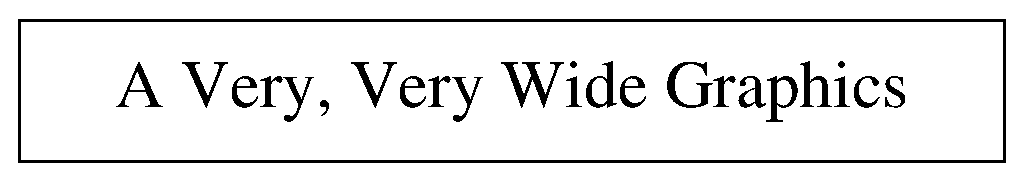
\includegraphics[width=\linewidth]{wide.eps} 
\caption{This is a wide figure} 
\end{narrow} 
\end{figure}
\end{Verbatim}

这里给定宽度参数为~\cmd{linewidth}~使得图形的宽度和~\texttt{narrow}~环境
的宽度相等。若给定宽度参数为~\cmd{textwidth}~会使图形的宽度和原来的
正文宽度一样。

当使用边注时,可能希望宽图形精确延伸到边注的边界(使得图形的宽度为
~\texttt{\bs textwidth}$+$\texttt{\bs marginparwidth}$+$%
\texttt{\bs marginparsep})。这时,可以定义一新长度~\texttt{\bs marginwidth}~
并将它设为~\texttt{\bs marginparwidth}$+$\texttt{\bs marginparsep}。
例如:
\begin{Verbatim}[xleftmargin=1cm]
\newlength{\marginwidth} 
\setlength{\marginwidth}{\marginparwidth} 
\addtolength{\marginwidth}{\marginparsep}
\end{Verbatim}
接着在~\cmd{begin\{narrow\}}~中使用~\texttt{-\bs marginwidth}~来达到目的。

\subsection{双面版式中的宽图形}

在使用双面版式排版时,页面左右的边空因奇偶页而取不同的值,
且使用宽图形时常常希望图形延伸到装订的那一边(奇数页的左边,
偶数页的右边)。在这种情形下,需要使用~\pai{ifthen}~宏包提供的
~\ci{ifthenelse}~命令来根据图形出现在奇数页或偶数页而使用不同的命令。
例如:
\begin{Verbatim}[xleftmargin=1cm]
\usepackage{ifthen}
...
\newlength{\marginwidth}
\setlength{\marginwidth}{\marginparwidth}
\addtolength{\marginwidth}{\marginparsep}
\begin{figure} 
\ifthenelse{\isodd{\pageref{fig:wide}}}% 
{% BEGIN ODD-PAGE FIGURE 
\begin{narrow}{0in}{-\marginwidth} 
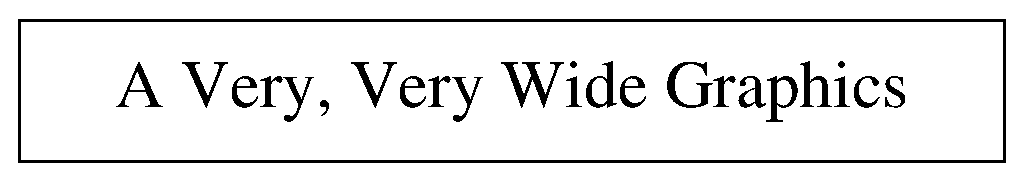
\includegraphics[width=\linewidth]{wide.eps}
\caption{Figure Caption} 
\label{fig:wide} 
\end{narrow} 
}% END ODD-PAGE FIGURE 
{% BEGIN EVEN-PAGE FIGURE 
\begin{narrow}{-\marginwidth}{0in} 
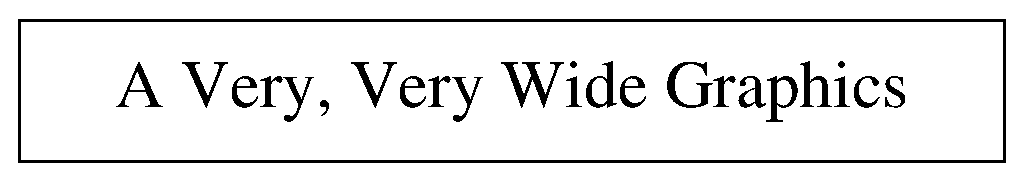
\includegraphics[width=\linewidth]{wide.eps} 
\caption{Figure Caption} 
\label{fig:wide} 
\end{narrow} 
}% END EVEN-PAGE FIGURE 
\end{figure}
\end{Verbatim}
结果如图~\ref{fig:wide}。由于~\cmd{ifthenelse}~使用命令~\cmd{pageref}~
作为输入,所以需要~\LaTeX{}~运行足够的次数后才能正确地排出。

\noindent{\CJKfamily{hei}注:}如果使用了~\pai{hyperref}~宏包,
上例中的~\cmd{pageref}~应替换为~\ci{hypergetpageref}~。

\newlength{\marginwidth}
\setlength{\marginwidth}{\marginparwidth}
\addtolength{\marginwidth}{\marginparsep}

\begin{figure}[hbp] 
	\ifthenelse{\isodd{\hypergetpageref{fig:wide}}}% 
	{% BEGIN ODD-PAGE FIGURE 
		\begin{narrow}{0in}{-\marginwidth} 
			
\includegraphics[width=\linewidth]{wide}
			\caption{Figure Caption}  
			\label{fig:wide}  
		\end{narrow}  
	}% END ODD-PAGE FIGURE 
	{% BEGIN EVEN-PAGE FIGURE 
		\begin{narrow}{-\marginwidth}{0in} 
			
\includegraphics[width=\linewidth]{wide} 
			\caption{Figure Caption} 
			\label{fig:wide} 
		\end{narrow} 
	}% END EVEN-PAGE FIGURE
\end{figure}

\section{横排的图形}

\noindent 在一竖排版的文档中,有三种方法来得到横排的图形。
\begin{enumerate}
	\item \pai{lscape}~宏包提供了一个~\ei{landscape}~环境,将纸张的左
	边界作为页面的顶部,使得在此环境中的文本,表格和图形都被
	横排。
	\item \pai{rotating}~宏包提供了一个~\ci{sidewaysfigure}~环境,与
	~\texttt{figure}~环境相似,只是其中的图形被横排。
	\item \pai{rotating}~宏包提供了一个~\ci{rotcaption}~命令,与
	~\cmd{caption}~命令相似,只是标题被横排。
\end{enumerate}

\noindent 以上三中方法的区别:
\begin{itemize}
	\item 方法~1~和~2~将横排的图形放到单独的一页上,而方法~3~则生成一个
	并不需要单独一页来放置的浮动对象。
	\item 方法~2~只是将其中的图形横排,而方法~1~则将位于~\texttt{landscape}~
	环境中的任何文本,图形和表格都横排在一页中。~\texttt{landscape}~
	环境具有分页的能力,可连续生成多个横排页面
	\realfootnote{~\texttt{landscape}~环境能很好的与~\pai{longtable}~
		宏包配合,从而得到连续多页横排的超长表格。}。
	\item 使用方法~2~得到的整页的图形可以浮动以求得最佳排版效果,而方法~1~
	得到的图形是不能浮动的\realfootnote{在~\texttt{landscape}~环境
		中声明的浮动图形只能在横排页中浮动。}。
	\item 因为方法~1~和~3~使用~\texttt{figure}~环境,所以它们可以和
	~\textsf{endfloat}~宏包(见第~\ref{sec:endfloat}~节)一起使用。
\end{itemize}

\subsection{Landscape~~环境}\label{ssec:landscape}

\textsf{landscape}~宏包(包括在标准的~\LaTeX{}~图形宏包套件中)定义
了~\texttt{landscape}~环境,允许在竖排版的文档中放置横排页。
横排页被旋转使得竖排页的左边界为其顶部。

输入命令~\cmd{begin\{landscape\}}~使得所有未处理的竖排的浮动对象
被排出并开始横排页,同样地,输入命令~\cmd{end\{landscape\}}~使得所
有未处理的横排的浮动对象被排出并重新回到竖排状态。

所有位于~\texttt{landscape}~环境中的内容都会被横排。如果只有
包含一个浮动图形环境
\begin{Verbatim}[xleftmargin=1cm]
\begin{landscape} 
\begin{figure} 
\centering 
\includegraphics[width=4in]{graphic.eps} 
\caption{Landscape Figure} 
\end{figure} 
\end{landscape}
\end{Verbatim}
这时会得到如图~\ref{fig:landscape}~所示的横排图形。不过,由于
~\texttt{landscape}~开始一新页,可能会导致页面出现很大空白。
如同此页 :)

\begin{landscape} 
	\begin{figure} 
		\centering
		\resizebox{4in}{!}{\usebox{\graphic}}
		\caption{Landscape Figure}\label{fig:landscape}
	\end{figure} 
\end{landscape}

\subsection{Sidewaysfigure~~环境}\label{ssec:sidewaysfigure}

\textsf{rotating}~宏包提供了~\texttt{sidewaysfigure}~环境来生成
横排的图形。例如:
\begin{Verbatim}[xleftmargin=1cm]
\begin{sidewaysfigure} 
\centering 
\includegraphics[width=4in]{graphic.eps} 
\caption{Sidewaysfigure Figure} 
\end{sidewaysfigure}
\end{Verbatim}
得到图~\ref{fig:sidewaysfigure}。

\begin{sidewaysfigure}
	\centering
	\resizebox{4in}{!}{\usebox{\graphic}}
	\caption{Sidewaysfigure Figure}\label{fig:sidewaysfigure}
\end{sidewaysfigure}

与~\texttt{landscape}~环境不同的是,由~\texttt{sidewaysfigure}~得到
的图形可在竖排页中浮动以避免导致出现过多空白的页面。相反~\texttt{landscape}~
环境则有更大的灵活性,允许横排页中有文本,表格和图形等。

\texttt{sidewaysfigure}~排出的图形的外观缺省由文档使用~\texttt{oneside}~
还是~\texttt{twoside}~版式所决定。
\begin{itemize}
	\item 当使用~\texttt{oneside}~时,图形的底部面向竖排页的右边界。
	\item 当使用~\texttt{twoside}~时,图形的底部面向竖排页的外边界。
\end{itemize}
在调入~\textsf{rotating}~是使用宏包选项可以改变上述缺省行为。
如:
\begin{Verbatim}[xleftmargin=1cm]
\usepackage[figuresleft]{rotating}
\end{Verbatim}
使得用~\texttt{sidewaysfigure}~排出的图形的底部面向竖排页的左边界(无论
是~\texttt{oneside}~还是~\texttt{twoside}~)。同样,
\begin{Verbatim}[xleftmargin=1cm]
\usepackage[figuresright]{rotating}
\end{Verbatim}
使得用~\texttt{sidewaysfigure}~排出的图形的底部面向竖排页的右边界。

\subsection{Rotcaption~~命令}

用第~\ref{sec:landscape}~节和第~\ref{sec:sidewaysfigure}~节的方法
得到的横排图形都是放在一单独的横排页上的。不过对于比较小的图形来说,
显然没有必要。这种情况下,可以利用~\textsf{rotating}~宏包中的
~\cmd{rotcaption}~来得到小的横排图形。例如:
\begin{Verbatim}[xleftmargin=1cm]
\begin{figure} 
\centering 
\begin{minipage}[c]{1in} 
\includegraphics[angle=90,width=\textwidth]{graphic.eps}
\end{minipage} 
\begin{minipage}[c]{0.5in} 
\rotcaption{Rotcaption Caption} 
\label{fig:rotcaption} 
\end{minipage} 
\end{figure}
\end{Verbatim}
得到图~\ref{fig:rotcaption}。

\begin{figure} 
	\centering 
	\begin{minipage}[c]{1in}
		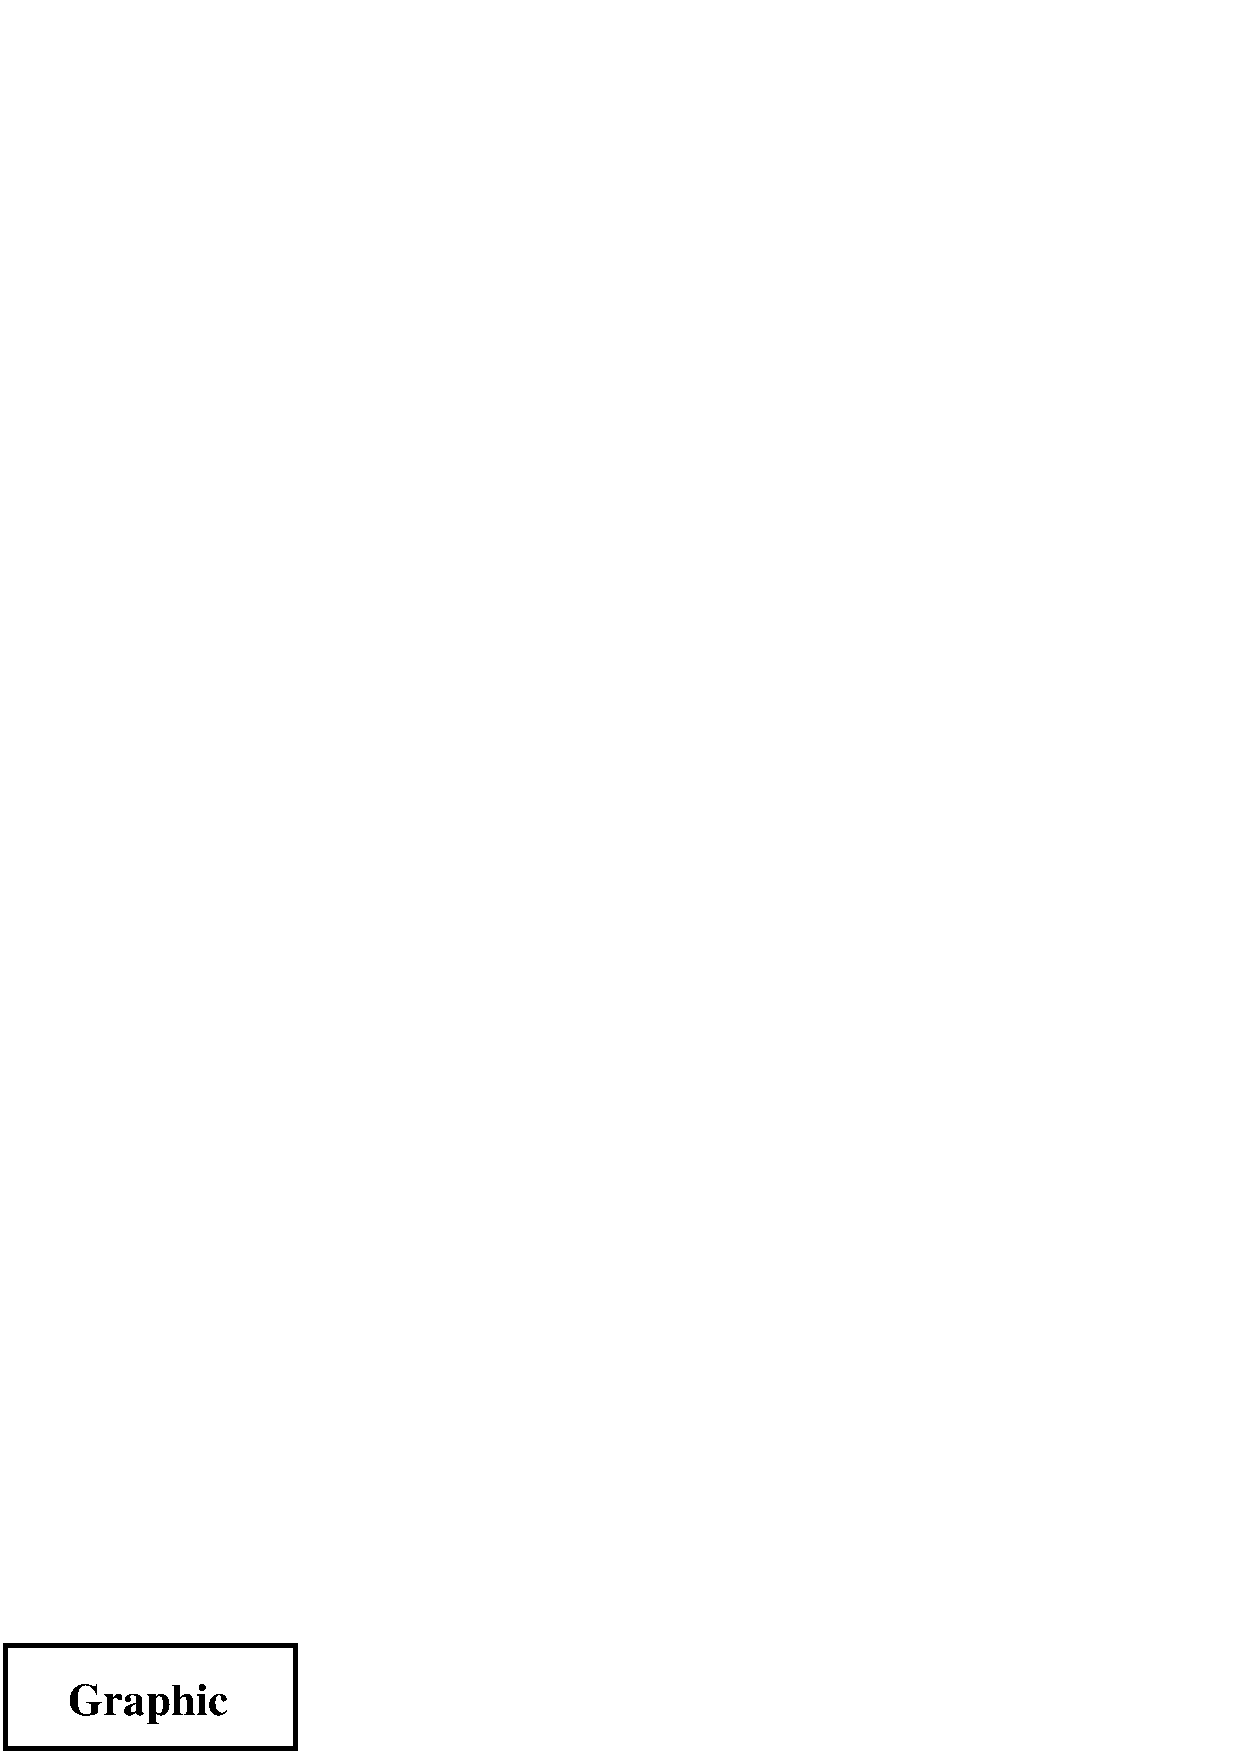
\includegraphics[angle=90,width=\textwidth]{graphic}  
	\end{minipage}
	\begin{minipage}[c]{0.5in} 
		\rotcaption{Rotcaption Caption} 
		\label{fig:rotcaption} 
	\end{minipage}
\end{figure}

\cmd{rotcaption}~命令生成的标题总是旋转使得其底部面向页面的右边界。
与第~\ref{sec:landscape}~节和第~\ref{sec:sidewaysfigure}~节的方法
不同的是,~\cmd{rotcaption}~并不旋转图形。因此上例中的~\cmd{includegraphics}~
命令需要使用~\texttt{angle=90}~这一选项。

\section{标题在一边的图形}\label{sec:sidecaption}

一般来说,图形的标题放置在其上方或下方。本章将介绍怎样将标题放置在
图形的旁边\realfootnote{因为~\textsf{float}~宏包定义的~\texttt{figure}~环境
	中,标题固定在图形的下方,因此无法使用它来得到置于图形旁边的标题。
	只要没有声明~\cmd{restylefloat}~命令,其它的~\textsf{float}~宏包的
	命令都可使用。}。第~\ref{sec:leftcaption}~节介绍了将标题置于图形左侧的
方法,同样地也可将标题置于图形的右侧。对于双面版式的文档,第
~\ref{sec:bindcaption}~节介绍了将标题置于图形内侧(奇数页中为图形的
左侧,偶数页中为图形的右侧)的方法。

\subsection{图形左侧标题}\label{ssec:leftcaption}

\cmd{caption}~命令一般将标题置于图形或表格的下方。可以利用小页
环境来欺骗~\cmd{caption}~命令,从而使它把标题放在图形的一侧。
例如命令:
\begin{Verbatim}[xleftmargin=1cm]
\begin{figure} 
\centering 
\begin{minipage}[c]{.45\textwidth} 
\centering 
\caption{Caption on the Side} 
\label{fig:side:caption} 
\end{minipage}%
\begin{minipage}[c]{.45\textwidth} 
\centering 
\includegraphics[width=\textwidth]{graphic.eps} 
\end{minipage} 
\end{figure}
\end{Verbatim}
得到如图~\ref{fig:side:caption}~的结果。在小页之间加入像~\cmd{hfill}~
或~\cmd{hspace\{.05\bs textwidth\}}~的水平距离可能会更好些。

\begin{figure} 
	\centering 
	\begin{minipage}[c]{.45\textwidth} 
		\centering
		\caption{Caption on the Side} 
		\label{fig:side:caption} 
	\end{minipage}%
	\begin{minipage}[c]{.45\textwidth} 
		\centering 
		\resizebox{\textwidth}{!}{\usebox{\graphic}}
	\end{minipage}  
\end{figure}

图~\ref{fig:side:caption}~中标题和图形垂直居中。如果想让图形和标题
顶部对齐或底部对齐,可参见第~\ref{sec:minivalign}节。

\subsection{图形内侧标题}\label{ssec:bindcaption}

上节图~\ref{fig:side:caption}~中将标题放在图形的左侧,而对于双面版式
的文档,常常会希望将标题置于图形的内侧。这时可用~\textsf{ifthen}~宏包
的~\cmd{ifthenelse}~命令来指定对奇数页和偶数页所使用的不同代码。例如:
\begin{Verbatim}[xleftmargin=1cm]
\usepackage{ifthen} 
... 
\begin{figure} 
\centering 
\ifthenelse{\isodd{\pageref{fig:side:caption}}} 
{% BEGIN ODD-PAGE FIGURE 
\begin{minipage}[c]{.45\textwidth} 
\centering 
\caption{Caption on the Side} 
\label{fig:side:caption} 
\end{minipage}% 
\hspace{0.05\textwidth}% 
\begin{minipage}[c]{.45\textwidth} 
\includegraphics[width=\textwidth]{graphic.eps} 
\end{minipage}% 
}% END ODD-PAGE FIGURE
{% BEGIN EVEN-PAGE FIGURE 
\begin{minipage}[c]{.45\textwidth} 
\includegraphics[width=\textwidth]{graphic.eps} 
\end{minipage}% 
\hspace{0.05\textwidth}% 
\begin{minipage}[c]{.45\textwidth} 
\centering 
\caption{Caption on the Side} 
\label{fig:side:caption} 
\end{minipage}% 
}% END EVEN-PAGE FIGURE 
\end{figure}
\end{Verbatim}
生成的图形其标题总在图形的内侧。

\subsection{Sidecap~~宏包}\label{ssec:sidecap}

利用前面量节介绍的方法可以得到标题在一侧的图形。如果希望有更多的灵活性,
那么使用~\pai{sidecap}~宏包将更为简单方便。

当在~\textsf{sidecap}~宏包提供的~\ei{SCfigure}~
环境中使用~\cmd{caption}~命令时,标题会被自动地放置于图形的一侧。
例如:
\begin{Verbatim}[xleftmargin=1cm]
\usepackage{sidecap} 
... 
\begin{SCfigure} 
\includegraphics[width=3in]{graphic.eps} 
\caption{This is a SCfigure} 
\end{SCfigure}
\end{Verbatim}
结果如图~\ref{fig:sidecap}~所示。

\begin{SCfigure} 
	\resizebox{3in}{!}{\usebox{\graphic}}
	\caption{This is a SCfigure}
	\label{fig:sidecap}
\end{SCfigure}

\noindent\textsf{sidecap}~宏包在用~\cmd{usepackage}~调入时有下面四个可选项:
\begin{description}
	\item [outercaption] 标题在偶数页中出现在左侧,奇数页中出现在右侧。
	这也是~\textsf{sidecap}~宏包的缺省选项。
	\item [innercaption] 标题在偶数页中出现在右侧,奇数页中出现在左侧。
	\item [leftcaption]  标题总出现在左侧。
	\item [rightcaption] 标题总出现在右侧。
\end{description}

\noindent\texttt{Scfigure}~环境包括下面两个可选参数:
\begin{itemize}
	\item 第一个可选参数指定标题对于图形的相对宽度。一个大的值(如~100)会让
	标题使用最大可能的宽度。缺省为~1。
	\item 第二个可选参数指定图形的浮动位置选项。如~\texttt{[htp]}~或
	~\texttt{[!ht]}~等,详见第~ref{sec:figplacement}~节。
\end{itemize}

\section{奇偶页中的图形}

图形环境的浮动放置算法不能控制图形出现在奇数页还是偶数页。要达到
控制浮动图形的奇数或偶数页放置,必须使用~\textsf{afterpage}~宏包
的~\cmd{afterpage}~命令和~\textsf{ifthen}~宏包的~\cmd{ifthenelse}~
命令。

将图形置于~\texttt{figure}~环境,可能会使得在偶数页中声明的图形被浮动到奇数页
中。反之,使用第~\ref{chap:nonfloat}~章中定义的~\cmd{figcaption}~命令
则可在不用~\texttt{figure}~环境的情况下生成图形。
\begin{Verbatim}[xleftmargin=1cm]
\makeatletter 
\newcommand\figcaption{\def\@captype{figure}\caption} 
\makeatother
\end{Verbatim}

使用~\cmd{ifthenelse}~命令可用来将出现在奇数页上的图形放到下一偶数页
上。这需要重复一次插图命令,一次是对应于下一页为奇数页的情况,另一次
则对应于下一页为偶数页的情况。为简便起见,首先定义一个~\ci{leftfig}~命令:
\begin{Verbatim}[xleftmargin=1cm]
\newcommand\leftfig{% 
\vspace*{\fill}% 
\centering 
\includegraphics{graphic.eps} 
\figcaption{This is on the left (even) page.} 
\vspace*{\fill}\newpage}
\end{Verbatim}
接下来就可以用这个新定义的命令和~\cmd{afterpage},\cmd{ifthenelse}~命令一起
来生成一幅只出现在偶数页上的图形。
\begin{Verbatim}[xleftmargin=1cm]
\afterpage{\clearpage% 
\ifthenelse{\isodd{\value{page}}}% 
{\afterpage{\leftfig}}% 
{\leftfig}}
\end{Verbatim}

\noindent{\CJKfamily{hei}几点说明:}
\begin{itemize}
	\item 欲使图形只出现在奇数页上,掉换一下~\cmd{ifthenelse}~的参数顺序即可。
	\begin{Verbatim}
	\afterpage{\clearpage% 
	\ifthenelse{\isodd{\value{page}}}% 
	{\leftfig}}%
	{\afterpage{\leftfig}}
	\end{Verbatim}
	\item 使用~\cmd{value\{page\}}~而不是~\cmd{pageref}~的好处是它总是正确的。
	相反,~\cmd{pageref}~只有在~\LaTeX{}~的交叉引用收敛时才正确。
	\item 当图形较大时,可能会出现在图形中间(图形与标题之间)分页的情况。
	这时可将它放到一个小页环境中以保持它的完整性。
	\begin{Verbatim}
	\newcommand\leftfig{% 
	\vspace*{\fill}% 
	\begin{minipage}{\textwidth} 
	\centering 
	\includegraphics{graphic.eps} 
	\figcaption{This is on the left (even) page.} 
	\end{minipage} 
	\vspace*{\fill}\newpage}
	\end{Verbatim}
	\item \cmd{afterpage}~命令在极少数情况下会造成一个~``lost float''~的错误,
	这时将~\cmd{clearpage}~从~\cmd{ifthenelse}~前去掉可能会有所帮助。
	\begin{Verbatim}[xleftmargin=1cm]
	\afterpage{\ifthenelse{\isodd{\value{page}}}% 
	{\afterpage{\leftfig}}% 
	{\leftfig}}
	\end{Verbatim}
	\item 在上面的例子中,图形是占据完整的一偶数页的。要将其置于偶数页的顶部,
	修改或去掉~\cmd{vspace*\{\bs fill\}}~和~\cmd{newpage}~命令。
	\begin{Verbatim}
	\newcommand\leftfig{% 
	\centering 
	\includegraphics{graphic.eps} 
	\figcaption{This is at the top of the left (even) page.} 
	\vspace{\floatsep}}
	\end{Verbatim}
\end{itemize}

\subsection{迎面页图形}

在双面版式的文档中,为消除浮动图形间差别,常常希望将图形放在迎面页
(\texttt{facing page})上。为达到这一目的,仍须使用与前两节中相似的
方法。为简单起见,定义命令~\ci{facingfigures}~如下:
\begin{Verbatim}[xleftmargin=1cm]
\newcommand\facingfigures{% 
\vspace*{\fill}% 
\centering 
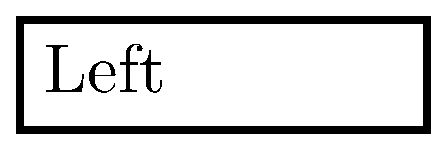
\includegraphics{left.eps} 
\figcaption{This is on the left (even) page.} 
\vspace*{\fill}\newpage\vspace*{\fill}% 
\centering 
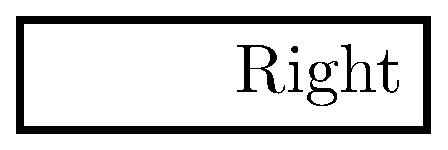
\includegraphics{right.eps} 
\figcaption{This is on the right (odd) page.} 
\vspace*{\fill}\newpage}
\end{Verbatim}
这时可用~\cmd{facingfigures}~与~\cmd{afterpage},\cmd{ifthenelse}~一起
来生成迎面页图形。
\begin{Verbatim}[xleftmargin=1cm]
\afterpage{\clearpage% 
\ifthenelse{\isodd{\value{page}}}% 
{\afterpage{\facingfigures}}% 
{\facingfigures}}
\end{Verbatim}

\section{盒子中的图形}

\noindent 盒子中的图形通常指下面两种情形:
\begin{itemize}
	\item 图形在盒子中,但其标题在盒子之外。
	\item 图形及其标题都在盒子中。
\end{itemize}

将某一对象置于盒子中的最基本的方法就是把它放到~\ci{fbox}~命令中,这样
会将该对象用一长方形的框围起来。~\pai{fancybox}~宏包提供了不同式样的盒子。

\subsection{图形在盒子中}

把~\cmd{includegraphics}~命令放到~\cmd{fbox}~中会使所插入的图形置于
一个带框盒子中。例如:
\begin{Verbatim}[xleftmargin=1cm]
\begin{figure} 
\centering 
\fbox{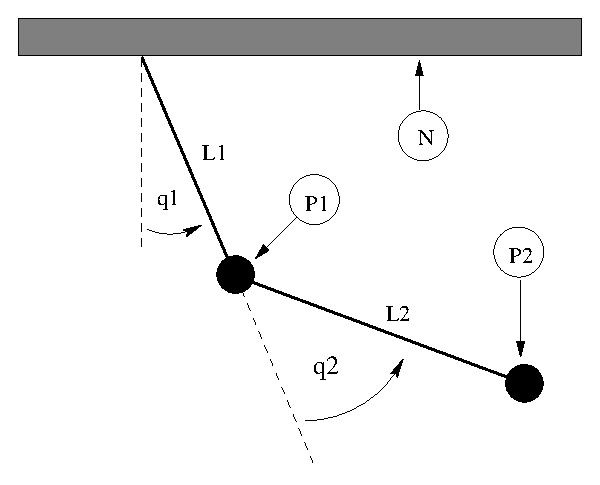
\includegraphics[totalheight=2in]{pend.eps}} 
\caption{Box Around Graphic, But Not Around Caption} 
\label{fig:boxed_graphic} 
\end{figure}
\end{Verbatim}
如图~\ref{fig:boxed_graphic}所示,图形被置于一带框盒子中。

\clearpage

\begin{figure} 
	\centering 
	\fbox{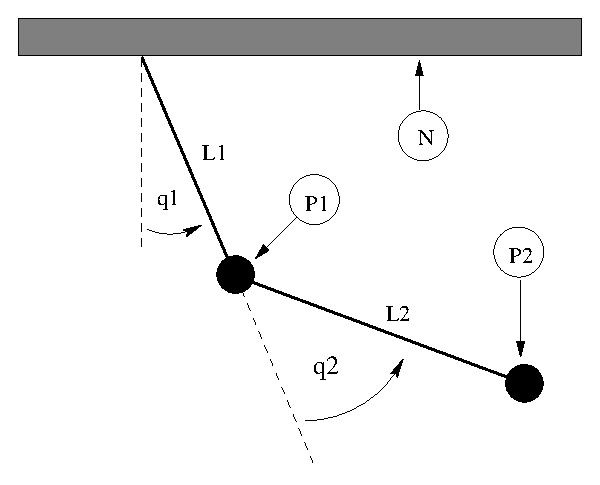
\includegraphics[totalheight=2in]{pend}}
	\caption{Box Around Graphic, But Not Around Caption} 
	\label{fig:boxed_graphic}
\end{figure}

\subsection{图形与标题均在盒子中}

要将图形与标题均置于盒子中,也许有人想当然的以为把~\cmd{caption}~
命令也放到~\cmd{fbox}~命中就可以了。然而,由于~\cmd{caption}~命令
只能在段落模式中使用,而~\cmd{fbox}~命令中的内容是在~LR~模式中被处理
的\realfootnote{\LaTeX{}~使用三种模式,~LR~,段落模式和数学模式。},
所以这样做是不能达到目的的。

因为小页环境的内容和~\cmd{parbox}~命令都使在段落模式中处理,所以将
~\cmd{fbox}~命令的内容放到小页环境或~\cmd{parbox}~命令中,就可以把
~\cmd{caption}~包含在~\cmd{fbox}~中。由于小页环境和~\cmd{parbox}~命令
都必须给出它们的宽度,故没有直接的办法让~\cmd{fbox}~和图形及其标题一样
宽。 例如下列命令:
\begin{Verbatim}[xleftmargin=1cm]
\begin{figure} 
\centering 
\fbox{ 
\begin{minipage}{4 in} 
\centering 
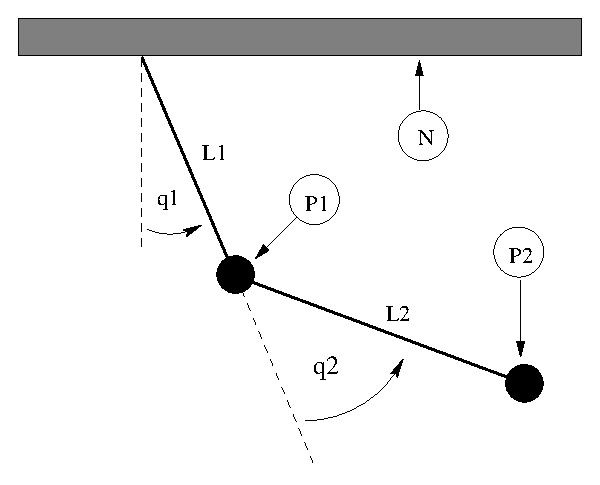
\includegraphics[totalheight=2in]{pend.eps} 
\caption{Box Around Figure Graphic and Caption} 
\label{fig:boxed_figure} 
\end{minipage} } 
\end{figure}
\end{Verbatim}
得到图~\ref{fig:boxed_figure},其中图形与标题都置于盒子中。

\begin{figure} 
	\centering 
	\fbox{ 
		\begin{minipage}{4 in} 
			\centering 
			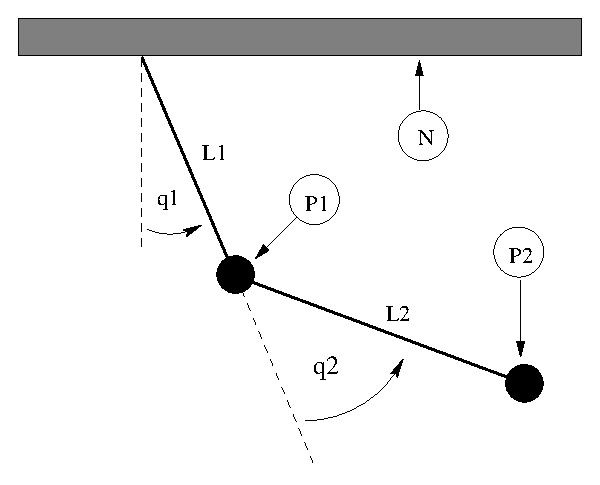
\includegraphics[totalheight=2in]{pend}
			\caption{Box Around Figure Graphic and Caption} 
			\label{fig:boxed_figure} 
	\end{minipage} }
\end{figure}

一般通过不断的尝试修改来确定小页环境的宽度从而使得盒子能够恰好
围住图形和标题。下面的这些方法可以避免枯燥麻烦的尝试修改。
\begin{enumerate}
	\item 选择一个确定的小页的宽度,使得图形的宽度与其相同。
	\begin{Verbatim}
	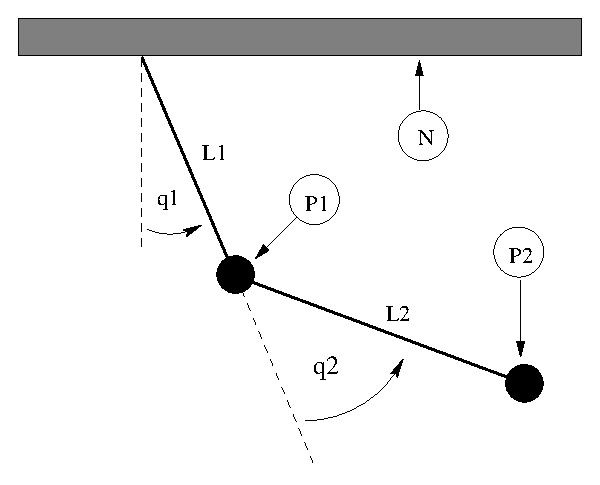
\includegraphics[width=\textwidth]{pend.eps}
	\end{Verbatim}
	\item 当指定图形的高度时,适当的小页的宽度可以通过把图形放到一个
	盒子中,然后计算盒子的宽度来得到。
	\begin{Verbatim}
	\newsavebox{\mybox} 
	\newlength{\mylength} 
	\sbox{\mybox}{\includegraphics[height=3in]{file.eps}} 
	\settowidth{\mylength}{\usebox{\mybox}} 
	\begin{figure}
	\centering 
	\fbox{ 
	\begin{minipage}{\mylength} 
	\centering 
	\usebox{\mybox} 
	\caption{Box Around Figure Graphic and Caption} 
	\label{fig:boxed_figure} 
	\end{minipage} } 
	\end{figure}
	\end{Verbatim}
	\item 为保证标题只有一行,可以使用~\ci{settowidth}~命令来估计标题
	的宽度并将其作为小页的宽度。
	\begin{Verbatim}
	\newlength{\mylength} 
	\settowidth{\mylength}%
	{Figure XX: Box Around Figure Graphic and Caption} 
	\fbox{ \begin{minipage}{\mylength} 
	...
	\end{Verbatim}
\end{enumerate}

\subsection{定制~~fbox~~的参数}

在图~\ref{fig:boxed_graphic}~和~\ref{fig:boxed_figure}~中,盒子由
厚为~0.4pt~的直线围成,在框线和图形之间有~3pt~的距离。这些维数值
都可以通过使用~\cmd{setlength}~命令设置~\LaTeX{}~的长度变量
~\cmd{fboxrule}~和~\cmd{fboxsep}~来修改。例如命令:
\begin{Verbatim}[xleftmargin=1cm]
\begin{figure} 
\centering 
\setlength{\fboxrule}{3pt} 
\setlength{\fboxsep}{1cm} 
\fbox{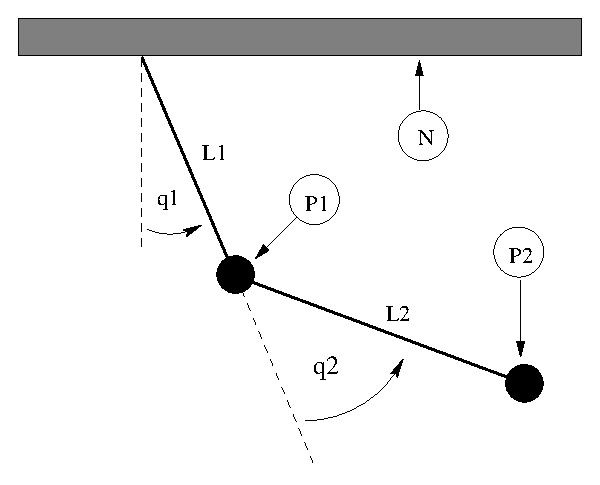
\includegraphics[totalheight=2in]{pend.eps}} 
\caption{Graphic with Customized Box} 
\label{fig:boxed_custom} 
\end{figure}
\end{Verbatim}
使得盒子的边框线厚为~3pt~且其与图形间的距离为~1~厘米。如图
~\ref{fig:boxed_custom}~所示。

\begin{figure} 
	\centering 
	\setlength{\fboxrule}{3pt} 
	\setlength{\fboxsep}{1cm} 
	\fbox{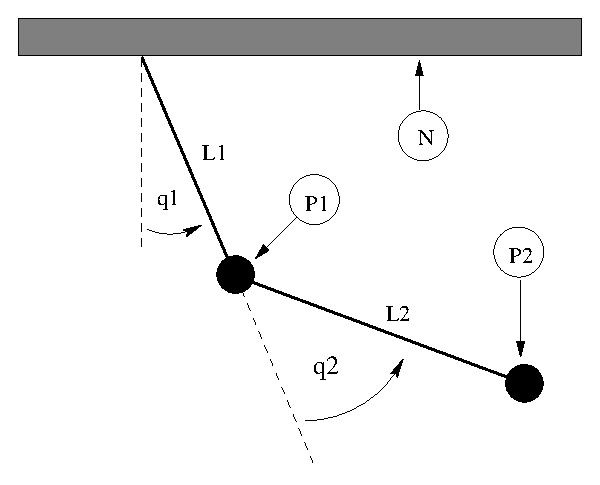
\includegraphics[totalheight=2in]{pend}}
	\caption{Graphic with Customized Box} 
	\label{fig:boxed_custom} 
\end{figure}

\subsection{fancybox~~宏包}

在图~\ref{fig:boxed_graphic},\ref{fig:boxed_figure}~和~\ref{fig:boxed_custom}~
中,用~\cmd{fbox}~命令将图形包围在标准的长方形框盒子中。要想使用不同类型的
盒子,可使用~\pai{fancybox}~宏包。它提供了~\ci{shadowbox}, \ci{doublebox},
\ci{ovalbox}~和~\ci{Ovalbox}~四个命令来生成不同形状的盒子。

\begin{table}
	\newcommand{\tbltt}[1]{\textcolor{blue}{\texttt{#1}}}
	\renewcommand{\arraystretch}{1.2}
	\centering
	\topcaption{\textsf{FancyBox} Commands}\label{tab:fancybox}
	
	\begin{tabular}{|m{4cm}|>{\CJKfamily{kai}}m{10cm}|}
		
		\hline
		\centering\tbltt{\bs shadowbox\{Example\}} 
		
		\centering\shadowbox{Example}  &
		\begin{itemize}
			\item 盒子边框线厚度为~\cmd{fboxrule}
			\item 盒子阴影厚度为~\cmd{shadowsize}~(缺省为~4pt)。
		\end{itemize} \\
		\hline
		\centering\tbltt{\bs doublebox\{Example\}} 
		
		\centering\doublebox{Example} &
		\begin{itemize}
			\item 内框线厚为~.75\cmd{fboxrule}。 
			\item 外框线厚为~1.5\cmd{fboxrule}。
			\item 内外框之间的距离为~1.5\cmd{fboxrule}$+$0.5pt。
		\end{itemize} \\
		\hline
		\centering\tbltt{\bs ovalbox\{Example\}}
		
		\centering\ovalbox{Example} &
		\begin{itemize}
			\item 盒子边框线厚度为~\cmd{thinlines}。
			\item 使用~\ci{cornersize\{x\}}~四个角的直径设为~\texttt{x}~乘以盒子宽和高
			之间较小的那个。缺省为~0.5。
			\item 使用~\cmd{cornersize*\{x\}}~命令直接将四个角的直径设为~\texttt{x}。
			如~\cmd{cornersize*\{1cm\}}~将四个角的直径设为~1~厘米。
		\end{itemize} \\
		\hline
		\centering\tbltt{\bs Ovalbox\{Example\}} 
		
		\centering\Ovalbox{Example}  &
		除了盒子边框线厚度为~\cmd{thicklines}~外,均与~\cmd{ovalbox}~一样。\\
		\hline
	\end{tabular}
\end{table}

如同~\cmd{fbox}~命令一样,这些盒子命令中的内容与边框间距由~\LaTeX{}~长度
~\cmd{fboxsep}~控制。长度~\cmd{shadowsize}~可用~\cmd{setlength}~命令来设定。
而~\cmd{ovalbox}~和~cmd{Ovalbox}~命令中的边框线厚度对应于~\texttt{picture}~
环境中的~\cmd{thinlines}~和~\cmd{thicklines}~的值,由于它们不是长度,所以
无法用~\cmd{setlength}~来设定。这两个值依赖于当前字体的大小和形状,缺省
分别为~0.4pt~和~0.8pt。例如:
\begin{Verbatim}[xleftmargin=1cm]
\begin{figure} 
\centering 
\shadowbox{ 
\begin{minipage}{3.5 in} 
\centering 
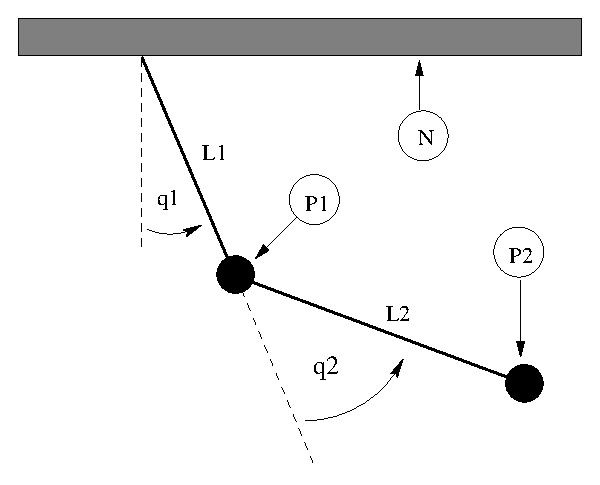
\includegraphics[totalheight=2in]{pend.eps} 
\caption{Shadowbox Around Entire Figure} 
\label{fig:boxed_fancy} 
\end{minipage} } 
\end{figure}
\end{Verbatim}
用一个带阴影的盒子将图形与标题包围起来,如图~\ref{fig:boxed_fancy}~所示。

\begin{figure} 
	\centering 
	\shadowbox{ 
		\begin{minipage}{3.5 in} 
			\centering 
			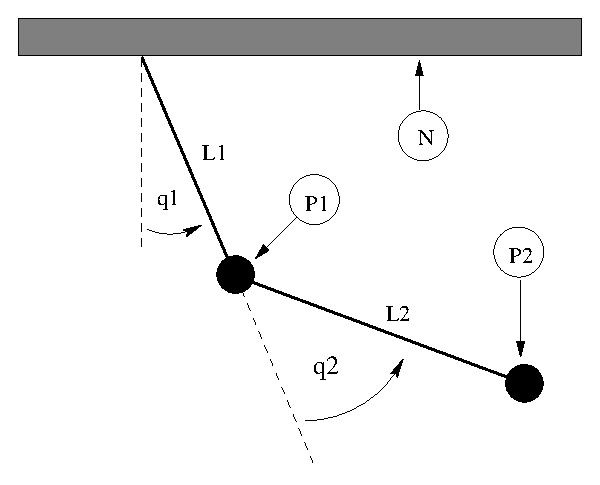
\includegraphics[totalheight=2in]{pend} 
			\caption{Shadowbox Around Entire Figure} 
			\label{fig:boxed_fancy} 
	\end{minipage} } 
\end{figure}

\section{并列的图形}\label{sec:sidebyside}

使图形并列所需的命令依赖于用户到底想怎样来组织图形。本章主要讨论
三种常见的并列图形。
\begin{enumerate}
	\item 多个图形并列于一个图形环境中。
	\item 多个并列的浮动图形,如图~\ref{fig:side:a}~和~\ref{fig:side:b}。
	\item 一图形环境中各个子图的平行排列。如子图~\ref{fig:subfig:a}~和
	~\ref{fig:subfig:b}~并列于图~\ref{fig:subfig}~中。
\end{enumerate}

本章中将用下列两种方法来生成上述三种并列图形。
\begin{enumerate}
	\item 连续使用~\cmd{includgraphics}~命令。
	\item 并列的小页环境,其中每个都包含一~\cmd{includegraphics}~命令。
\end{enumerate}
理解第~\ref{sec:sidefigure}~节的内容在构造多个并列的浮动图形
非常重要。并列的浮动图形是通过将盒子(\cmd{incudegraphics}~或小页)平行
放置在一条线上来得到的。

\subsection{一图形环境中的并列图形}\label{ssec:sidegraphics}

连续使用多个~\cmd{includgraphics}~命令是生成并列图形的最简单的方法,
仅管使用并列的小页环境能够让那些并列的图形更好地对齐。

下面的命令:
\begin{Verbatim}[xleftmargin=1cm]
\begin{figure} 
\centering 
\includegraphics[width=1in]{graphic.eps}% 
\hspace{1in}% 
\includegraphics[width=2in]{graphic.eps} 
\caption{Two Graphics in One Figure} 
\end{figure}
\end{Verbatim}
得到如图~\ref{fig:sidegraphics}~的并列图形。~4~英寸宽,居中放置。
其中的~\cmd{hspace}~命令可用~\cmd{hfill}~来代替,使得将图形推向页
面的两边边界(见第~\ref{sec:hspace}~节)。

\begin{figure} 
	\centering 
	\resizebox{1in}{!}{\usebox{\graphic}}%
	\hspace{1in}%
	\resizebox{2in}{!}{\usebox{\graphic}}
	\caption{Two Graphics in One Figure} 
	\label{fig:sidegraphics}
\end{figure}

将~\cmd{includegraphics}~命令放到小页环境中可以让用户更好地控制
图形的对齐方式。例如:
\begin{Verbatim}[xleftmargin=1cm]
\begin{figure} 
\centering 
\begin{minipage}[c]{0.5\textwidth} 
\centering 
\includegraphics[width=1in]{graphic.eps} 
\end{minipage}% 
\begin{minipage}[c]{0.5\textwidth} 
\centering 
\includegraphics[width=2in]{graphic.eps} 
\end{minipage} 
\caption{Centers Aligned Vertically} 
\end{figure}
\end{Verbatim}
生成图~\ref{fig:minipagegraphics}~,其中的图形是中间对齐的。

\begin{figure} 
	\centering 
	\begin{minipage}[c]{0.5\textwidth} 
		\centering 
		\includegraphics[width=1in]{graphic}
	\end{minipage}% 
	\begin{minipage}[c]{0.5\textwidth} 
		\centering 
		\includegraphics[width=2in]{graphic}
	\end{minipage} 
	\caption{Centers Aligned Vertically} 
	\label{fig:minipagegraphics}
\end{figure}

对于这个例子,需要注意以下几点:
\begin{itemize}
	\item 如同其它的~\LaTeX{}~对象一样,小页在放置时,它的参考点和当前基线对齐。
	缺省小页使用~\texttt{[c]}~选项,将参考点置于其竖直方向的中点。其它的选项
	如~\texttt{[t],[b]}~等的含义与使用技巧可参见第~\ref{sec:minivalign}~节。
	\item 在第一个~\cmd{end\{minipage\}}~后面的~\%~防止在两个小页盒子中间
	加上一个字符间距,详见第~\ref{sec:hspace}~节。
	\item 当几个并列小页的宽度之和没有达到~1.0\cmd{textwidth}~时,可用
	~\cmd{hspace}~或~\cmd{hfill}~来确定水平间距,详见第~\ref{sec:hspace}~节。
\end{itemize}

\subsection{并列的浮动图形}\label{ssec:sidefigure}

在上一节中,通过在一个图形环境中使用多个小页环境从而得到一个由
多幅图形组成的浮动图形。若将~\cmd{caption}~命令放到每个小页环境
中,则每个小页环境就生成一浮动图形。例如:
\begin{Verbatim}[xleftmargin=1cm]
\begin{figure} 
\begin{minipage}[t]{0.5\linewidth} 
\centering 
\includegraphics[width=1in]{graphic.eps} 
\caption{Small Box} 
\label{fig:side:a} 
\end{minipage}% 
\begin{minipage}[t]{0.5\linewidth} 
\centering 
\includegraphics[width=1.5in]{graphic.eps} 
\caption{Big Box} 
\label{fig:side:b} 
\end{minipage} 
\end{figure}
\end{Verbatim}
生成图~\ref{fig:side:a}~和~\ref{fig:side:b}。尽管上面的命令
只使用了一个~\texttt{figure}~环境,但由于每个小页中都包含一
个~\cmd{caption}~命令,所以仍然得到两个浮动图形。

\begin{figure} 
	\begin{minipage}[t]{0.5\linewidth} 
		\centering 
		\includegraphics[width=1in]{graphic}
		\caption{Small Box} 
		\label{fig:side:a} 
	\end{minipage}% 
	\begin{minipage}[t]{0.5\linewidth} 
		\centering 
		\includegraphics[width=1.5in]{graphic}
		\caption{Big Box} 
		\label{fig:side:b} 
	\end{minipage} 
\end{figure}

在图~\ref{fig:side:a}~和~\ref{fig:side:b}中,并列的小页环境使用了
~\texttt{[t]}~选项,使得两幅图形的基线对齐。这对于非旋转的图形
没有任何问题,而且使得两标题的顶部对齐。不过,如果图形的底部
不对齐的话(如其中一图形被旋转),就会发生问题。例如:
\begin{Verbatim}[xleftmargin=1cm]
\begin{figure} 
\centering 
\begin{minipage}[t]{.33\textwidth} 
\centering 
\includegraphics[width=2cm]{graphic.eps} 
\caption{Box with a Long Caption} 
\end{minipage}% 
\begin{minipage}[t]{.33\textwidth} 
\centering 
\includegraphics[width=2cm,angle=-30]{graphic.eps} 
\caption{Rotated Box} 
\end{minipage}% 
\end{figure}
\end{Verbatim}
生成图~\ref{fig:mininonrot}~和~\ref{fig:minirot},我们可以看到这里
两幅图形的标题并不对齐。而若只使用小页的~\texttt{[b]}~选项,会使得标题
的最后一行对齐,并不能解决问题。

\begin{figure} 
	\centering 
	\begin{minipage}[t]{.33\textwidth} 
		\centering 
		\includegraphics[width=2cm]{graphic} 
		\caption{Box with a Long Caption}\label{fig:mininonrot} 
	\end{minipage}%   
	\begin{minipage}[t]{.33\textwidth} 
		\centering 
		\includegraphics[width=2cm,angle=-30]{graphic} 
		\caption{Rotated Box}\label{fig:minirot} 
	\end{minipage}% 
\end{figure}

一种解决办法是在小页环境中把图形和标题分开放到两行中:第一行放置图形,
第二行放置标题。例如:
\begin{Verbatim}[xleftmargin=1cm]
\begin{figure} 
\centering 
\begin{minipage}[b]{.33\textwidth} 
\centering 
\includegraphics[width=2cm]{graphic.eps} 
\end{minipage}% 
\begin{minipage}[b]{.33\textwidth} 
\centering 
\includegraphics[width=2cm,angle=-30]{graphic.eps} 
\end{minipage}\\[-10pt] 
\begin{minipage}[t]{.33\textwidth} 
\caption{Box with a Long Caption} 
\end{minipage}% 
\begin{minipage}[t]{.33\textwidth} 
\caption{Rotated Box} 
\end{minipage}% 
\end{figure}
\end{Verbatim}
生成的图~\ref{fig:mininonrot:a}~和~\ref{fig:minirot:a}~中,图形的基
线和标题的第一行分别对齐。

\begin{figure}
	\centering
	\begin{minipage}[b]{.33\textwidth}
		\centering
		\includegraphics[width=2cm]{graphic}
	\end{minipage}%
	\begin{minipage}[b]{.33\textwidth}\label{fig:mininonrot:a}
		\centering
		\includegraphics[width=2cm,angle=-30]{graphic}
	\end{minipage}\\[-10pt]
	\begin{minipage}[t]{.33\textwidth}
		\caption{Box with a Long Caption}
	\end{minipage}%
	\begin{minipage}[t]{.33\textwidth}
		\caption{Rotated Box}\label{fig:minirot:a}
	\end{minipage}%
\end{figure}

\noindent在这个例子中,需要注意:
\begin{itemize}
	\item 在最后一幅图后面用~\cmd{\bs}~来断行,~\cmd{\bs}~的参数项
	~\texttt{[-10pt]}~使得图形与标题之间的距离比当前行距
	减少~\texttt{10pt}。这样做是让图形和标题更接近些,用户也可
	自己选用合适的值。
	\item 包含图形的小页使用~\texttt{[b]}~选项,使得它们的参考点为
	其最后一行的基线。
	\item 包含标题小页使用~\texttt{[t]}~选项,使得它们的参考点为
	其第一行的基线。
	\item 任何一个~\cmd{label}~命令都必须和它相应的~\cmd{caption}~
	命令在同一个小页中。
\end{itemize}

\subsection{并列的子图形}\label{ssec:sidesubfigure}

在某些情况下,有时会希望将并列的图形组成一组,而其中的每一幅图
都保持其独立性。~pai{subfigure}~宏包的~\ci{subfigure}~命令将这一
组做为一幅图形,其中的每一幅图做为子图形。例如:
\begin{Verbatim}[xleftmargin=1cm]
\begin{figure} 
\centering 
\subfigure[Small Box with a Long Caption]{ 
\label{fig:subfig:a} %% label for first subfigure 
\includegraphics[width=1.0in]{graphic.eps}} 
\hspace{1in} 
\subfigure[Big Box]{ 
\label{fig:subfig:b} %% label for second subfigure 
\includegraphics[width=1.5in]{graphic.eps}} 
\caption{Two Subfigures} 
\label{fig:subfig} %% label for entire figure 
\end{figure}
\end{Verbatim}
生成图~\ref{fig:subfig}。这里使用~\LaTeX{}~的引用命令~\cmd{ref\{fig:subfig:a\}}~
会得到~\ref{fig:subfig:a},~\cmd{ref\{fig:subfig:b\}}~得到~\ref{fig:subfig:b},
~\cmd{ref\{fig:subfig\}}~得到~\ref{fig:subfig}。

\begin{figure} 
	\centering 
	\subfigure[Small Box with a Long Caption]{ 
		\label{fig:subfig:a} %% label for first subfigure 
		\resizebox{1in}{!}{\usebox{\graphic}}} 
	\hspace{1in} 
	\subfigure[Big Box]{ 
		\label{fig:subfig:b} %% label for second subfigure 
		\resizebox{1.5in}{!}{\usebox{\graphic}}}
	\caption{Two Subfigures} 
	\label{fig:subfig} %% label for entire figure 
\end{figure}

像其它的并列图形一样,子图也可以在小页环境中使用。而且在一些情况下,
这样做还能更方便的得到理想的图形间距。例如:
\begin{Verbatim}[xleftmargin=1cm]
\begin{figure} 
\subfigure[Small Box with a Long Caption]{ 
\label{fig:mini:subfig:a} %% label for first subfigure 
\begin{minipage}[b]{0.5\textwidth} 
\centering 
\includegraphics[width=1in]{graphic.eps} 
\end{minipage}}% 
\subfigure[Big Box]{ 
\label{fig:mini:subfig:b} %% label for second subfigure 
\begin{minipage}[b]{0.5\textwidth} 
\centering 
\includegraphics[width=1.5in]{graphic.eps} 
\end{minipage}} 
\caption{Minipages Inside Subfigures} 
\label{fig:mini:subfig} %% label for entire figure 
\end{figure}
\end{Verbatim}
得到图~\ref{fig:mini:subfig},其中包括两个子图~\ref{fig:mini:subfig:a}~
和~\ref{fig:mini:subfig:b}。

\begin{figure} 
	\subfigure[Small Box with a Long Caption]{ 
		\label{fig:mini:subfig:a} %% label for first subfigure 
		\begin{minipage}[b]{0.5\textwidth} 
			\centering 
			\includegraphics[width=1in]{graphic} 
	\end{minipage}}% 
	\subfigure[Big Box]{ 
		\label{fig:mini:subfig:b} %% label for second subfigure 
		\begin{minipage}[b]{0.5\textwidth} 
			\centering 
			\includegraphics[width=1.5in]{graphic} 
	\end{minipage}} 
	\caption{Minipages Inside Subfigures} 
	\label{fig:mini:subfig} %% label for entire figure 
\end{figure}

图~\ref{fig:mini:subfig}~中的子图标题比图~\ref{fig:subfig}~中的要宽一些。
这是因为子图标题的宽度和子图的宽度相同,图~\ref{fig:subfig}~中的子图
只包含图形,而图~\ref{fig:mini:subfig}~中的子图包含了宽度为
~\texttt{0.5\bs textwidth}~的小页。

子图的标记有两种形式:
\begin{enumerate}
	\item 一种是出现在子图的下面作为标题的一部分。这通过命令~\ci{@thesubfigure}~
	来生成。
	\item 另一种是在使用~\cmd{ref}~命令的时候出现。这通过将命令~\ci{p@subfigure}~
	的输出处理后传递给~\cmd{thesubfigure}~命令来生成。
\end{enumerate}

上面的这些命令使用~\texttt{subfigure}~计数器和~\cmd{thefigure}~命令。
子图的标记的格式由下面的命令来控制。
\begin{itemize}
	\item 命令~\cmd{thefigure}~印出当前图形的编号。
	\item 计数器~\texttt{subfigure}~记录子图的编号,命令~\cmd{alph\{subfigure\}}~
	将计数器~\texttt{subfigure}~的值用小写字母印出,而
	命令~\cmd{roman\{subfigure\}}~则是用小写罗马数字印出(有关印出
	计数器值的命令可参见文献~\cite[第~98~页]{Leslie}~和
	~\cite[第~446~页]{Michel}。)。
	\item 命令~\cmd{thesubfigure}~缺省使用小写字母,如~(a),(b)~等。
	\item 命令~\cmd{@thesubfigure}~缺省为~\cmd{thesubfigure}\cmd{space},即在
	标题标记和文本之间加上一个空白。
	\item 命令~\cmd{p@subfigure}~缺省为~\cmd{thefigure}。
\end{itemize}

如果改变子图标题的标记,字体等的缺省值,可参见文献~\cite{subfigure}。下面
给出几个简单的例子:\marginpar{\CJKfamily{kai}\bfseries 子图的例子}
\begin{itemize}
	\item 若想让子图标题标记使用小写罗马数字如~(i), (ii)等,~\cmd{ref}~命令的结果
	如~12i, 12ii~等,可使用下面的命令(最好放在导言区中)
	\begin{Verbatim}
	\renewcommand{\thesubfigure}{\roman{subfigure}} 
	\makeatletter 
	\renewcommand{\@thesubfigure}{(\thesubfigure)\space} 
	\renewcommand{\p@subfigure}{\thefigure} 
	\makeatother
	\end{Verbatim}
	\item 若想让子图标题标记使用阿拉伯数字如~12.1:, 12.2:~等,~\cmd{ref}~命令的结果
	如~12.1, 12.2~等,可使用下面的命令
	\begin{Verbatim}
	\renewcommand{\thesubfigure}%
	{\thefigure.\arabic{subfigure}} 
	\makeatletter 
	\renewcommand{\@thesubfigure}{\thesubfigure:\space} 
	\renewcommand{\p@subfigure}{} 
	\makeatother
	\end{Verbatim}
\end{itemize}

缺省情况下,用~\cmd{listoffigures}~命令生成的图形目录中只包括图形,
而不包括子图。要想在图形目录中包括子图,要在~\cmd{listoffigures}~
命令前加上~\cmd{setcounter\{lofdepth\}\{2\}}。

需要说明的是,由于~\LaTeX{}~的变化,导致目前版本(\texttt{\textit{3/95}})
的~\textsf{subfigure}~宏包在图形目录的子图输入项开始部分都加上
``numberline1''。将下面的代码加到导言区中就可以解决这一问题。
\begin{Verbatim}[xleftmargin=1cm]
\makeatletter 
\renewcommand{\@subcaption}[2]{% 
\begingroup 
\let\label\@gobble 
\def\protect{\string\string\string}% 
\xdef\@subfigcaptionlist{% 
\@subfigcaptionlist,% 
{\numberline {\@currentlabel}% 
\noexpand{\ignorespaces #2}}}% 
\endgroup 
\@nameuse{@make#1caption}{\@nameuse{@the#1}}{#2}} 
\makeatother
\end{Verbatim} 

\section{堆叠图形}

在第~\ref{chap:sidebyside}~章中,通过将几个盒子并排放置在
一行中来得到并列图形。堆叠图形(stacked graphics)也可用同样的
方法来生成。例如:
\begin{Verbatim}[xleftmargin=1cm]
\begin{figure} 
\centering 
\begin{minipage}[b]{0.3\textwidth} 
\centering 
\includegraphics[width=1in]{graphic.eps} 
\caption{Caption 1}
\end{minipage}% 
\hspace{0.04\textwidth}% 
\begin{minipage}[b]{0.3\textwidth} 
\centering 
\includegraphics[width=1in]{graphic.eps} 
\caption{Caption 2} 
\end{minipage}\\[20pt] 
\begin{minipage}[b]{0.3\textwidth} 
\centering 
\includegraphics[width=1in]{graphic.eps} 
\caption{Caption 3} 
\end{minipage}% 
\hspace{0.04\linewidth}% 
\begin{minipage}[b]{0.3\textwidth} 
\centering 
\includegraphics[width=1in]{graphic.eps} 
\caption{Caption 4} 
\end{minipage}% 
\hspace{0.04\linewidth}% 
\begin{minipage}[b]{0.3\textwidth} 
\centering 
\includegraphics[width=1in]{graphic.eps} 
\caption{Caption 5} 
\end{minipage} 
\end{figure}
\end{Verbatim}
得到图~\ref{fig:stacked:a}-\ref{fig:stacked:e}。其中在~``Caption2''~小页后
的~\texttt{\bs\bs[20pt]}~命令得到一增加了~20pt~的行距。

\begin{figure} 
	\centering 
	\begin{minipage}[b]{0.3\textwidth} 
		\centering 
		\includegraphics[width=1in]{graphic} 
		\caption{Caption 1}\label{fig:stacked:a}
	\end{minipage}% 
	\hspace{0.04\textwidth}% 
	\begin{minipage}[b]{0.3\textwidth} 
		\centering 
		\includegraphics[width=1in]{graphic} 
		\caption{Caption 2} \label{fig:stacked:b}
	\end{minipage}\\[20pt] 
	\begin{minipage}[b]{0.3\textwidth} 
		\centering 
		\includegraphics[width=1in]{graphic} 
		\caption{Caption 3} \label{fig:stacked:c}
	\end{minipage}% 
	\hspace{0.04\linewidth}% 
	\begin{minipage}[b]{0.3\textwidth} 
		\centering 
		\includegraphics[width=1in]{graphic} 
		\caption{Caption 4} \label{fig:stacked:d}
	\end{minipage}% 
	\hspace{0.04\linewidth}% 
	\begin{minipage}[b]{0.3\textwidth} 
		\centering 
		\includegraphics[width=1in]{graphic} 
		\caption{Caption 5} \label{fig:stacked:e}
	\end{minipage} 
\end{figure}

\section{图形与表格的平行排列}\label{sec:figuretable}

在第~\ref{chap:sidebyside}~章中,通过在一个~\texttt{figure}~环境中使用多个
~\cmd{caption}~命令来得到并列的多个图形。同样地,在一个~\texttt{table}~
环境中使用多个~\cmd{caption}~命令可将多个表格平行排列。
若想使表格和图形平行排列在一起,可使用第~\ref{chap:nonfloat}~中定义
的命令~\cmd{figcaption}~和~\cmd{tabcaption}。
例如下面的命令:
\begin{Verbatim}[xleftmargin=1cm]
\begin{figure}[htb] 
\begin{minipage}[b]{0.5\textwidth} 
\centering 
\includegraphics[width=0.8\textwidth]{graphic.eps} 
\caption{This is a Figure by a Table} 
\label{fig:by:table} 
\end{minipage}% 
\begin{minipage}[b]{0.5\textwidth} 
\centering
\begin{tabular}{|c|c|} \hline 
Day & Data \\ \hline\hline 
Monday    & 14.6 \\ 
Tuesday   & 14.3 \\ 
Wednesday & 14.2 \\ 
Thursday  & 14.5 \\ 
Friday    & 14.9 \\ \hline 
\end{tabular} 
\tabcaption{This is a Table by a Figure} 
\label{table:by:fig} 
\end{minipage} 
\end{figure}
\end{Verbatim}
用一个~\texttt{figure}~环境生成了并排放置的图~\ref{fig:by:table}~和
表~\ref{table:by:fig}。

\begin{figure}[htb]
	\begin{minipage}[b]{0.5\textwidth}
		\centering
		\includegraphics[width=0.8\textwidth]{graphic} 
		\caption{This is a Figure by a Table} 
		\label{fig:by:table} 
	\end{minipage}% 
	\begin{minipage}[b]{0.5\textwidth} 
		\centering
		\begin{tabular}{|c|c|} \hline
			Day & Data \\ \hline\hline
			Monday    & 14.6 \\ 
			Tuesday   & 14.3 \\
			Wednesday & 14.2 \\ 
			Thursday  & 14.5 \\ 
			Friday    & 14.9 \\ \hline
		\end{tabular}
		\tabcaption{This is a Table by a Figure} 
		\label{table:by:fig} 
	\end{minipage} 
\end{figure}

因为~\LaTeX{}~允许图形的浮动不必考虑其前后表格的顺序,所以在
~\texttt{figure}~环境中使用命令~\cmd{tabcaption}~可能会将表格
放置到尚未处理的浮动图形前面。同理,在~\texttt{table}~环境中
使用命令~\cmd{figcaption}~可能会将图形放置到尚未处理的浮动图形前面。
这种情况下,可以在图形环境前使用~\cmd{FloatBarrier}~命令来清除
其前面尚未处理的浮动图形。

\section{图文混排}

在使用外部图形时,通常的是将其置于一个~\texttt{figure}~环境中,
由这一浮动环境来决定最后的位置是在页面的上方或下方。
但有的时候,许多使用者往往希望将图形放置在一个正文方格内,或者置
于页面的左右,也可能是在页面的的中间,四周包围者文本,
甚至放在文字的下方作为背景,或重叠放置。这时,前面所介绍的
只使用~\LaTeX{}~图形宏包套件就很难得到所希望的结果。本章将介绍几个
有用的图形宏包,可以让你很容易地得到上述特殊效果。

本章介绍的几个图形宏包均可从~\texttt{CTAN}~下载。如果你使用的
是~te\TeX{}~或~fp\TeX{},那么这些宏包已包括在内了,你所做的只
需是在文档中调用它们:
\begin{Verbatim}[xleftmargin=1cm]
\usepackage[选项]{宏包}
\end{Verbatim}
除了本章所介绍的宏包外,还有一些宏包也可完成同样的工作。
如~\pai{floatflt}~也可用来将图形置于文本段落的一边。
而所介绍的宏包中,也有未涉及的内容,进一步的研究
可阅读这些宏包所附的帮助文件。

\subsection{Wrapfig~~宏包}\label{ssec:wrapfig}

\intextsep=0pt
\begin{wrapfigure}{l}{25pt}
	\textcolor{blue}{\mbox{\bfseries\texttt{\PartSize W}}}
\end{wrapfigure} \noindent \texttt{rapfig}~宏包提供了一个
~\ei{wrapfigure}~环境\footnote{\pai{wrapfig}~也
	同时提供了一个~\ei{wraptable}~环境。}来排版窄小的图形,使得
该图形位于文本的一边,并使文本在其边上折行。

~\texttt{wrapfigure}的用法:

\noindent{%
	\color{morelight}{\shadowbox{\textcolor{blue}{\CJKfamily{kai}\texttt{%
					\bs begin\{wrapfigure\}\{行数\}[位置][超出长度]\{宽度\}<图形>\bs end\{wrapfigure
					\}}}}}}

\noindent 这里{\CJKfamily{kai} 行数}是指图形高度所占的文本行的数目。
如果不给出此选项,~\pai{wrapfig}~会自动计算。
{\CJKfamily{kai} 位置}是指图形相对于文本的位置,须给定下面四项的一个。
\begin{description}
	\item [\texttt{[r],[R]}] 表示图形位于文本的左边。
	\item [\texttt{[l],[L]}] 表示图形位于文本的右边。
	\item [\texttt{[i],[R]}] 表示图形位于页面靠里的一边(用在双面格式里)。
	\item [\texttt{[o],[O]}] 表示图形位于页面靠外的一边。
\end{description}
{\CJKfamily{kai} 超出长度}是指图形超出文本边界的长度,缺省为~0pt。
{\CJKfamily{kai} 宽度}则指图形的宽度。~\textsf{wrapfig}~会自动计算
图形的高度。不过,我们也可设定图形的高度,具体可见~\texttt{wrapfig.sty}~内
的说明。

\begin{wrapfigure}{r}{4.5cm}
	\includegraphics [width=4cm,clip]{tiger}
\end{wrapfigure}
\mbox{}在使用~\textsf{wrapfig}~时需要注意下面几点:

\begin{itemize}
	\item 在~\texttt{wrapfigure}~后必须紧接着输入段落文字,否则会出错。
	\item 不能在任何列表环境中使用~\texttt{wrapfigure},也不能在
	列表环境前后使用,除非两者之间有一空行或分段指令~\ci{par}。
	\item 如果将~\texttt{wrapfigure}~放在~\cmd{parbox}~或小页环境
	等分组中,文本折行必须在这些分组前结束。
	\item 在双栏页版式中不能使用~\texttt{wrapfigure}。
	\item 如果在~\texttt{wrapfigure}~中使用~\texttt{figure}~等
	浮动对象,它的编号有可能不正确。
	\item 如果在~\texttt{wrapfigure}~中使用~\texttt{table}~等浮动对象,
	它上下方的横线可能被忽略,必须自己再加入。
	\item 在折行的文本中,~\cmd{linewidth}~并没有改变。
\end{itemize}

\textsf{wrapfig}~还可用来放大段落的第一个字。本节的第一个字目~\texttt{W}~
就是使用如下命令来得到的:
\begin{Verbatim}[xleftmargin=1cm]
\newcommand{\PartSize}{\fontsize{1.5cm}{1.5cm}\selectfont}
\intextsep=0pt
\begin{wrapfigure}{l}{25pt}
\textcolor{blue}{\mbox{\texttt{\PartSize W}}}
\end{wrapfigure}
\noindent\texttt{rapfig}宏包提供了一个...
\end{Verbatim}

本节中的另一例子使用了如下命令:
\begin{Verbatim}[xleftmargin=1cm]
\begin{wrapfigure}{r}{4.5cm}
\includegraphics [width=4cm,clip]{tiger.ps}
\end{wrapfigure}
\mbox{}在使用\textsf{wrapfig}时需要注意下面几点:
\end{Verbatim}

\subsection{Picinpar~~宏包}\label{ssec:picinpar}

\pai{picinpar}~宏包定义了一个基本的环境~\ei{window},还有两个变体
~\ei{figwindow}~和~\ei{tabwindow}。允许在文本段落中打开一个``窗口'',
在其中放入图形、文字和表格等。这里我们主要讨论将图形放入文本段落
的用法,其它的用法可参考~\textsf{picinpar}~的说明。

\noindent{%
	\color{morelight}{\shadowbox{\textcolor{blue}{\CJKfamily{kai}\texttt{%
					\bs begin\{window\}[行数,对齐方式,内容,内容说明]\bs end\{window\}}}}}}

\noindent{%
	\color{morelight}{\shadowbox{\textcolor{blue}{\CJKfamily{kai}\texttt{%
					\bs begin\{figwindow\}[行数,对齐方式,图形,标题]\bs end\{figwindow\}}}}}}

\noindent 这里的{\CJKfamily{kai} 行数}是指``窗口''开始前的行数。
{\CJKfamily{kai} 对齐方式}是指在段落中``窗口''的对齐方式。缺省为~\texttt{l},
即左对齐。另外两种是~\texttt{c}~:居中和~\texttt{r}~:右对齐。
第三个参数是出现在``窗口''中的内容,这在~\texttt{figwindow}~中就是
要插入的图形。第四个参数则是对``窗口''内容的说明性文字,这在
~\texttt{figwindow}~中就是图形的标题。
下面是几个例子:

\begin{Verbatim}
\begin{window}[2,c,{\fcolorbox{morelight}{\shortstack{%
\color{yellow} 你在他乡 \\还 好 \\ 吗?}}},{}]
可是哈卜拉姆再聪明……
……可是我偏不喜欢。」
\end{window}
\end{Verbatim}

\CJKfamily{kai}
\begin{window}[2,c,{\fcolorbox{morelight}{yellow}{\CJKfamily{hei}{%
				\shortstack{你在他乡 \\还好 \\ 吗?}}}},{}]
	可是哈卜拉姆再聪明、再有学问,有一件事却是他不能解答的,因为包
	罗万有的「可兰经」上也没有答案;如果你深深爱著的人,却深深的爱上了
	别人,有甚麽法子?白马带著她一步步的回到中原。白马已经老了,只能慢
	慢的走,但终是能回到中原的。江南有杨柳、桃花,有燕子、金鱼……汉人中
	有的是英俊勇武的少年,倜傥潇洒的少年……但这个美丽的姑娘就像古高昌国
	人那样固执:「那都是很好很好的,可是我偏不喜欢。」
\end{window}

\begin{Verbatim}
\begin{figwindow}[1,r,{\mbox{%
\includegraphics[width=4cm]{tiger.ps}}},{Tiger}]
可是哈卜拉姆再聪明……
……可是我偏不喜欢。」
\end{window}
\end{Verbatim}

\begin{figwindow}[1,r,{\mbox{\includegraphics[width=4cm,clip]{tiger}}},%
	{Tiger}]
	可是哈卜拉姆再聪明、再有学问,有一件事却是他不能解答的,因为包
	罗万有的「可兰经」上也没有答案;如果你深深爱著的人,却深深的爱上了
	别人,有甚麽法子?白马带著她一步步的回到中原。白马已经老了,只能慢
	慢的走,但终是能回到中原的。江南有杨柳、桃花,有燕子、金鱼……汉人中
	有的是英俊勇武的少年,倜傥潇洒的少年……但这个美丽的姑娘就像古高昌国
	人那样固执:「那都是很好很好的,可是我偏不喜欢。」
\end{figwindow}

\begin{Verbatim}
\begin{figwindow}[1,c,{\mbox{%
\includegraphics[width=3cm]{tiger.ps}}},{Tiger}]
可是哈卜拉姆再聪明……
……可是我偏不喜欢。」
\end{window}
\end{Verbatim}

\begin{figwindow}[1,c,{\mbox{\includegraphics[width=3cm,clip]{tiger}}},%
	{Tiger}]
	可是哈卜拉姆再聪明、再有学问,有一件事却是他不能解答的,因为包
	罗万有的「可兰经」上也没有答案;如果你深深爱著的人,却深深的爱上了
	别人,有甚麽法子?白马带著她一步步的回到中原。白马已经老了,只能慢
	慢的走,但终是能回到中原的。江南有杨柳、桃花,有燕子、金鱼……汉人中
	有的是英俊勇武的少年,倜傥潇洒的少年……但这个美丽的姑娘就像古高昌国
	人那样固执:「那都是很好很好的,可是我偏不喜欢。」
\end{figwindow}

\CJKfamily{song}

在使用~\textsf{picinpar}~时要注意以下几点:
\begin{itemize}
	\item 不要在~\texttt{window}~环境中使用~\cmd{samepage}。
	\item 不要在~\texttt{window}~环境中使用~\cmd{footnote},代之在
	用~\ci{footnotemark}~标记角注,而将
	角注的内容在~\texttt{window}~环境外用~\ci{footnotetext}~来加入。
	\item 当使用~pai{epic}~宏包时,要确保在调入~\textsf{epic}~之前
	将它调入。
\end{itemize}

\subsection{Picins~宏包}\label{ssec:picins}

\pai{picins}~宏包定义了一个命令~\ci{parpic}命令,允许将
图形等~\LaTeX{}~对象放置在文本段落中。并且,设定适当的参数,
可把该对象置于一带框的盒子,有阴影的盒子等等。~\cmd{parpic}~
的用法如下:

\noindent{%
	\color{morelight}{\shadowbox{\textcolor{blue}{\CJKfamily{kai}\texttt{%
					\bs parpic(宽度,高度)(水平偏移,垂直偏移)[选项][位置]\{图形\}}}}}}

\noindent 上面除了{\CJKfamily{kai}图形}必须给出外,其余的均
可省略。如果宽度和高度均未给出,那么图形将以它的自然大小来
嵌入。{\CJKfamily{kai}选项}则可取以下的值:
\begin{description}
	\item [\CJKfamily{hei} 位置项] 只能为下面两个中的一个。
	\begin{description}
		\item [l] 将图形置于文本段落的左方(这也是缺省值)。
		\item [r] 将图形置于文本段落的右方。
	\end{description}
	\item [\CJKfamily{hei} 外观项] 只能为下面五个中的一个,可与上述位置项
	配合使用。
	\begin{description}
		\item [f] 将图形置于一个实框盒子中。
		\item [d] 将图形置于一个虚框盒子中。
		\item [o] 将图形置于一个圆角框盒子中。
		\item [s] 将图形置于一个具有阴影效果的盒子中。
		\item [x] 将图形置于一个具有立体效果的盒子中。
	\end{description}
\end{description}

\noindent{\CJKfamily{kai}位置}仅当给定的宽度和高度与
图形的实际大小相差很大的情况下才起作用。若水平或垂直偏移
已给出,那么此项也不起作用。缺省位置是将图形置于盒子的中央。
也可取以下的值:
\begin{description}
	\item [l] 将图形置于盒子的左方。
	\item [r] 将图形置于盒子的右方。
	\item [t] 将图形置于盒子的上方。
	\item [b] 将图形置于盒子的下方。
\end{description}

另外,~\textsf{picins}~宏包还提供了一些命令来控制图形
与文本的间距,图形外框的线宽等。详见~\textsf{picins}~宏包
所附的说明。下面是几个例子。

\CJKfamily{kai}
\hspace{-1.5cm}\begin{minipage}[b]{.5\textwidth}
	\parpic{\includegraphics[width=3cm,clip]{tiger}}
	仅当给定的宽度和高度与
	图形的实际大小相差很大的情况下才起作用。若水平或垂直偏移
	已给出,那么此项也不起作用。缺省位置是将图形置于盒子的中央。
	\par\vspace{0pt}
\end{minipage}%
\hspace{10pt}\begin{minipage}[b]{.5\textwidth}
	\begin{Verbatim}
	\parpic{%
	\includegraphics[width=3cm]%
	{tiger.ps}}
	仅当给定的宽度和高度与...
	\end{Verbatim}
	\par\vspace{0pt}
\end{minipage}

\hspace{-1.5cm}\begin{minipage}[b]{.5\textwidth}
	\parpic(3cm,3.5cm)[sr]{\includegraphics[width=2.5cm]{tiger}}
	仅当给定的宽度和高度与
	图形的实际大小相差很大的情况下才起作用。若水平或垂直偏移
	已给出,那么此项也不起作用。缺省位置是将图形置于盒子的中央。
	\par\vspace{0pt}
\end{minipage}%
\hspace{10pt}\begin{minipage}[b]{.5\textwidth}
	\begin{Verbatim}
	\parpic(3cm,3.5cm)[sr]{%
	\includegraphics[width=2.5cm]%
	{tiger.ps}}
	仅当给定的宽度和高度与...
	\end{Verbatim}
	\par\vspace{0pt}
\end{minipage}

\hspace{-1.5cm}\begin{minipage}[b]{.5\textwidth}
	\boxlength{10pt}%
	\parpic(3.5cm,4cm)[xr]{\includegraphics[width=3cm]{tiger}}
	仅当给定的宽度和高度与
	图形的实际大小相差很大的情况下才起作用。若水平或垂直偏移
	已给出,那么此项也不起作用。缺省位置是将图形置于盒子的中央。
	\par\vspace{0pt}
\end{minipage}%
\hspace{10pt}\begin{minipage}[b]{.5\textwidth}
	\begin{Verbatim}
	\boxlength{10pt}%
	\parpic(3.5cm,4cm)[xr]{%
	\includegraphics[width=3cm]%
	{tiger.ps}}
	仅当给定的宽度和高度与...
	\end{Verbatim}
	\par\vspace{0pt}
\end{minipage}

\CJKfamily{song}

\section{连续图形}

当两个相邻的图形含有关系较为密切的材料时,常常希望具有相同的
图形编号。因为计数器~\texttt{figure}~中记录了下一图形的编号,
所以可在图形环境前减低~\texttt{figure}~的值使得两幅图形具有
相同的编号。例如:
\begin{Verbatim}[xleftmargin=1cm]
\addtocounter{figure}{-1} 
\begin{figure}
\end{Verbatim}
不过,这样做会使得两幅图形无法被正确区分,导致~\LaTeX{}~的引用
等的混乱。

构造连续图形的最好的方法是使用~\textsf{subfigure}~宏包。
这样既可以使连续的几幅图形具有相同的编号,如~``{\CJKfamily{hei}图}~12'',
且其中的每幅图形也有自己的标记,如~``{\CJKfamily{hei}图}~12(a)''~等。
由于连续的子图位于不同的~\texttt{figure}~环境,所以在两个图形环境
之间,必须减低计数器~\texttt{figure}~的值。
\begin{Verbatim}[xleftmargin=1cm]
\addtocounter{figure}{-1} 
\end{Verbatim}
同时,必须在第二幅子图前将子图的计数器~\texttt{subfigure}~加一。
\begin{Verbatim}[xleftmargin=1cm]
\addtocounter{subfigure}{1}
\end{Verbatim}
例如下面的命令得到两个连续的子图。
\begin{Verbatim}[xleftmargin=1cm]
\begin{figure} 
\centering 
\subfigure[First Part]{% 
\label{fig:graphics:a}% label for subfigure 
\includegraphics[width=\textwidth]{wide.eps}}% 
\caption{Large Graphics}% 
\label{fig:graphics}% label for figure
\end{figure} 
\addtocounter{figure}{-1} 
\begin{figure} 
\addtocounter{subfigure}{1} 
\centering 
\subfigure[Second Part]{% 
\label{fig:graphics:b}% label for subfigure 
\includegraphics[width=\textwidth]{wide.eps}}% 
\caption{Large Graphics (con't)}% 
\end{figure}
\end{Verbatim}

\begin{figure} 
	\centering 
	\subfigure[First Part]{% 
		\label{fig:graphics:a}% label for subfigure 
		\includegraphics[width=\textwidth]{wide}}% 
	\caption{Large Graphics}%   
	\label{fig:graphics}% label for figure
\end{figure} 
\addtocounter{figure}{-1} 
\begin{figure} 
	\addtocounter{subfigure}{1} 
	\centering 
	\subfigure[Second Part]{% 
		\label{fig:graphics:b}% label for subfigure 
		\includegraphics[width=\textwidth]{wide}}% 
	\caption{Large Graphics (con't)}% 
\end{figure}

在这一例子中,每个图形环境中只有一个子图。而当像第~\ref{sec:sidesubfigure}~
节中那样每个图形环境中有多个子图,就需要根据第一个图形环境中子图的个数来
相应地调整计数器~\texttt{subfigure}~的增加值。另外,由于连续图形都是不
同的浮动对像,有可能不出现在连续的页面上。如果出现这种情况,可在最后
一幅连续图形后使用命令~\cmd{FloatBarrier}~来迫使~\LaTeX{}~将连续图形
放置在一起。

\endinput